\documentclass[11pt]{book}
\usepackage{titlesec}


{\Huge}
\usepackage[margin=1in]{geometry}
\usepackage{booktabs}
\usepackage{array}
\usepackage{float}
\usepackage{amsmath}
\usepackage{hyperref}
\usepackage{enumitem}
\usepackage{graphicx}
\usepackage{setspace}
\usepackage{tcolorbox}

\usepackage[
colorlinks=true,
linkcolor=blue,
citecolor=blue,
urlcolor=blue
]{hyperref}


\title{Data Analyst Technical Assessment}
\author{Analyst: Joevan M. Aliman}
\date{\today}

\begin{document}
	
	\maketitle
	\tableofcontents
	
\chapter*{About This Report}
\addcontentsline{toc}{chapter}{About This Report}

This report presents the results of a technical assessment of a digital advertising campaign dataset. The objective of the analysis is to evaluate campaign performance, identify the factors associated with advertising effectiveness, and provide data-driven recommendations to improve Return on Advertising Spend (ROAS).

To accommodate both business stakeholders and technical reviewers, the report is organized into two complementary sections.

\begin{itemize}
	\item \textbf{Main Report} — Presents the key business findings, interpretations, and recommendations in a concise, stakeholder-focused manner. Statistical results are summarized only where necessary to support business decisions.
	
	\item \textbf{Technical Appendices} — Provide the detailed analytical procedures supporting the main report, including the complete data quality assessment, data cleaning methodology, exploratory analyses, statistical assumption checks, hypothesis testing, and post-hoc analysis.
\end{itemize}

Readers interested primarily in the business implications may focus on the main report, while readers wishing to review the analytical methodology and supporting evidence may refer to the appendices.

This document also includes interactive cross-references. Figures, tables, equations, sections, and appendices references are hyperlinked throughout the report, allowing readers to navigate directly to the referenced content by clicking the corresponding reference.

\vspace{0.5cm}

\textbf{Software Used}

\begin{itemize}
	\item Python 3.13.5 (data cleaning, statistical analysis, and data processing)
	\item Visual Studio Code (Python development environment)
	\item Microsoft Power BI (data visualization and dashboard development)
	\item TeXstudio (report preparation using \LaTeX)
\end{itemize}
\renewcommand{\chaptername}{Task}
\chapter{Data Quality and Initial Exploratory Assessment}

Before conducting the performance analysis, the advertising campaign dataset was assessed to ensure that it was suitable for business decision-making. A comprehensive data quality assessment was performed, including verification of data types, duplicate records, missing values, logical consistency, and potential outliers. 

The complete details of these procedures are provided in Appendix~\ref{appendix:data_quality}.

\subsection{Data Cleaning Summary}

The data cleaning process consist of:

\begin{itemize}
	\item Verified variable data types
	
	\item Checked duplicate observations
	
	\item Removing observations(20 datapoints) with missing revenue.
	
	\item Retaining structurally missing Video Completion Rate values.
	
	\item Retaining valid view-through conversions.
	
	\item Removing observations(47 datapoints) with 0 clicks,impressions and purchases with non-zero purchase. 
	
	\item Addressed severe \texttt{Spend} outliers.
	
	
	
	
\end{itemize}

Overall, the dataset was determined to be sufficiently complete and reliable for subsequent analysis.

\subsection{Challenge}


The primary business challenges include:

\begin{itemize}
	\item Overall ROAS is substantially below the target value.
	\item Campaign performance varies considerably across advertising platforms, creative types, and product categories.
	\item Weekly ROAS has shown a declining trend, indicating decreasing advertising efficiency.
	\item Regional performance differences remain unclear.
	\item The impact of competitive events on campaign performance is uncertain.
	\item The effectiveness of different creative types and audience segments has not yet been established.
	\item Advertising spend must be reduced in underperforming areas while maintaining revenue growth.
\end{itemize}

\subsection{Performance Metrics}

We need numbers to evaluate campaign effectiveness. In that regard, four standard digital marketing performance metrics were considered.

\begin{table}[H]
	\centering
	\begin{tabular}{ll}
		\toprule
		Metric & Formula\\
		\midrule
		CTR & Clicks / Impressions\\
		CPC & Spend / Clicks\\
		CVR & Purchases / Clicks\\
		ROAS & Revenue / Spend\\
		\bottomrule
	\end{tabular}
	\caption{Calculated performance metrics.}
\end{table}

These metrics provide standardized measures of audience engagement, advertising efficiency, conversion effectiveness, and financial return.

\section{Initial Exploratory Assessment}

\subsection{Business Overview}

Following data cleaning, the overall Return on Advertising Spend (ROAS) is 0.96, which is below the company's target of 1.20. This indicates that the current advertising strategy is not generating sufficient revenue relative to advertising expenditure. Performance also varies across campaigns, platforms, creative types, product categories, and target audiences, suggesting opportunities to improve budget allocation and campaign effectiveness.

Since improving ROAS is the primary business objective, the subsequent analysis focuses on identifying the factors associated with both high- and low-performing advertising campaigns.

\subsection{Key Performance Metrics}

To evaluate advertising performance, the following baseline metrics were selected.

\begin{table}[H]
	\centering
	\begin{tabular}{lp{10cm}}
		\toprule
		Metric & Business Relevance\\
		\midrule
		Spend & Measures advertising investment and budget allocation.\\
		
		Revenue & Measures the financial return generated by advertising activities.\\
		
		ROAS & Primary indicator of advertising efficiency and campaign profitability.\\
		
		CTR & Measures audience engagement with advertisements.\\
		
		CPC & Measures the cost required to generate user engagement.\\
		
		CVR & Measures the effectiveness of converting engaged users into customers.\\
		
		\bottomrule
	\end{tabular}
	\caption{Baseline performance metrics used throughout the analysis.}
\end{table}

Together, these metrics provide a comprehensive view of advertising performance, covering investment, engagement, conversion, and financial return.

\subsection{Preliminary Insights}
I created a power BI dashboard(file is inside github repository) to summarize the ROAS to gives us a main idea of the campaign ad ROAS across different categorical variables.

\begin{figure}[h]
	\centering
	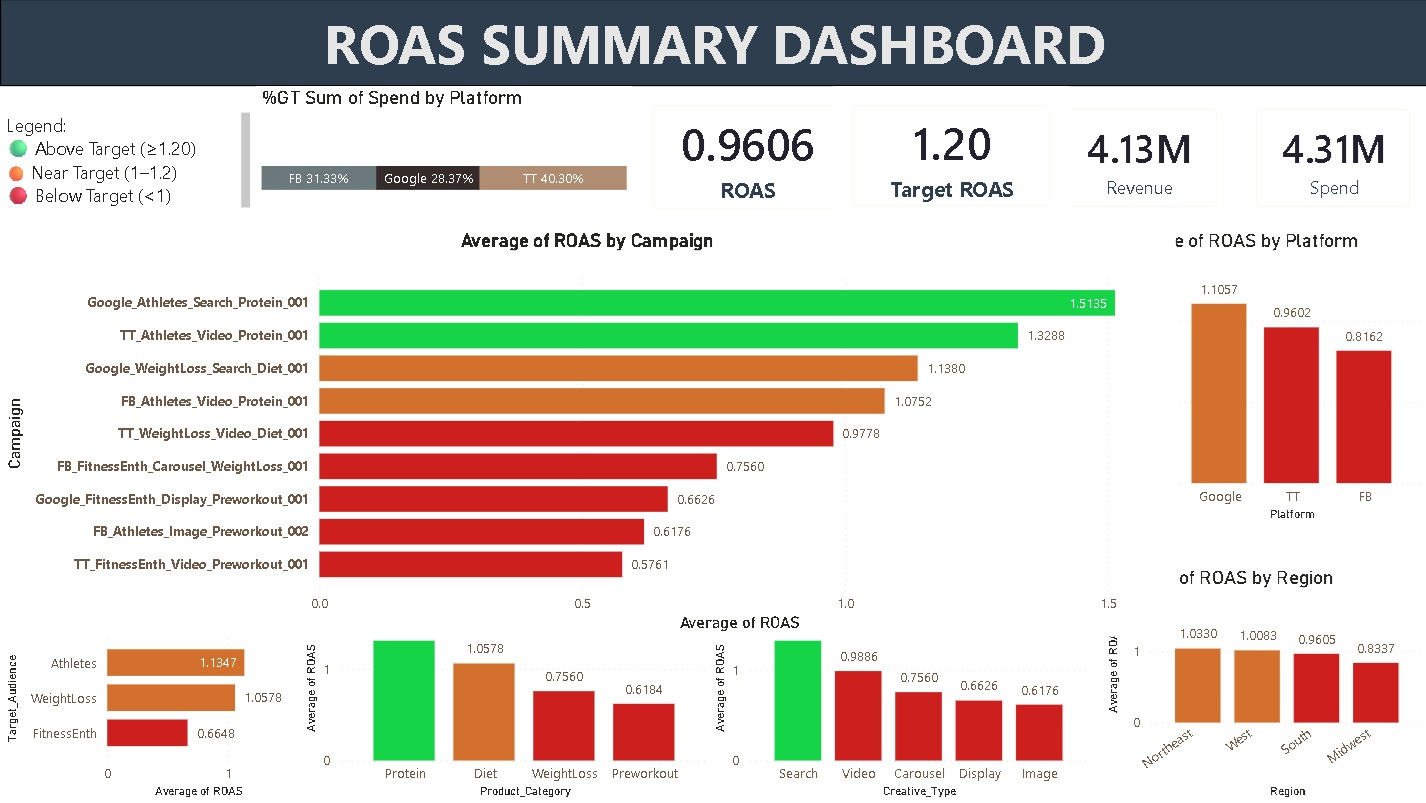
\includegraphics[width=1\textwidth]{images/roas_summary.jpg}
	\caption{ROAS Dashboard Summary}
	\label{fig:roas_summary}
\end{figure}

The executive dashboard provides an initial overview of advertising performance prior to detailed analysis. Several observations can be made:

\begin{itemize}
	
	\item Overall ROAS (0.96) remains below the business target of 1.20.
	
	\item Campaign performance varies substantially, with only a few campaigns exceeding the target ROAS.
	
	\item Google delivers the highest ROAS among advertising platforms, while Facebook records the lowest.
	
	\item Search creatives and Protein campaigns achieve the strongest advertising returns.
	
	\item Performance differences across regions are relatively small, whereas larger variation exists across creative types, product categories, and target audiences.
	
\end{itemize}

These observations establish a baseline understanding of current advertising performance and guide the subsequent analyses presented in Task 2.


\chapter{Performance Analysis}

The analyses presented in this chapter should be interpreted as exploratory rather than causal. Campaign cahracteristics including platform, product\_category, audience\_target, creative\_types, etc.. are not independently distributed across the dataset.

Consequently, observed performance differences cannot be attributed to any single factor in isolation. Instead, the objective of this chapter is to identify consistent performance patterns, prioritize areas for further investigation, and generate hypotheses to guide future optimization and controlled experiments.

However, descriptive statistics alone cannot determine whether these observed differences represent genuine performance differences or are simply the result of random variation. Therefore, statistical significance testing was performed before drawing business conclusions.

\section{Statistical Methodology}

The following statistical tests were used throughout the analysis:

\begin{enumerate}
	
	\item \textbf{Shapiro--Wilk Test}
	
	Used to assess whether the distribution of each performance metric follows a normal distribution. The results determined whether parametric statistical methods were appropriate for subsequent analyses.
	
	\textbf{Statistical Question:}
	\begin{itemize}
		\item \textit{Do the observed performance metrics satisfy the assumptions required for parametric statistical tests?}
	\end{itemize}
	
	\item \textbf{Levene's Test}
	
	Used to determine whether the variability (consistency) of a performance metric differs significantly across groups.
	
	\textbf{Business Question Answered:}
	\begin{itemize}
		\item \textit{Which business groups deliver more consistent advertising performance, and which exhibit greater variability or unpredictability?}
	\end{itemize}
	
	\item \textbf{Kruskal--Wallis Test}
	
	A non-parametric alternative to one-way ANOVA used to determine whether the distribution of a performance metric differs significantly across multiple groups. This test was selected because the normality assumption required for ANOVA was not satisfied.
	
	\textbf{Business Question Answered:}
	\begin{itemize}
		\item \textit{Do the observed differences in campaign performance across business groups (e.g., platforms, regions, creative types, product categories, and target audiences) represent genuine differences, or are they likely due to random variation?}
	\end{itemize}
	
	\item \textbf{Dunn's Post-hoc Test}
	
	Performed following a statistically significant Kruskal--Wallis test to identify which specific groups differ from one another while controlling for multiple comparisons.
	
	\textbf{Business Question Answered:}
	\begin{itemize}
		\item \textit{If significant differences exist, which specific business groups differ in their advertising performance?}
	\end{itemize}
	
\end{enumerate}

Together, these statistical procedures provide a systematic framework for validating assumptions, assessing performance consistency, determining whether differences are statistically significant, and identifying the specific groups responsible for those differences.

%%%%%%%%%%%%%%%%%%%%%%%%%%%%%%%%%%%%%%%%%%%%%%%%%%%%%%%%%%%%%%%%%%%%%%%%%%%%%%%%%%%%%%%%%%%%%%%%%%%%%%%%%%%%%%%%%%%%%%%%%%%%%%%%%%%%%%%%%%%%%%%%%%%%%%%%%%

\newpage
\section{Channel Performance Analysis}
Performance metrics across different channel/platforms was investigated and is shown in Fig. \ref{fig:metrics_by_platform}. 

\begin{figure}[h]
	\centering
	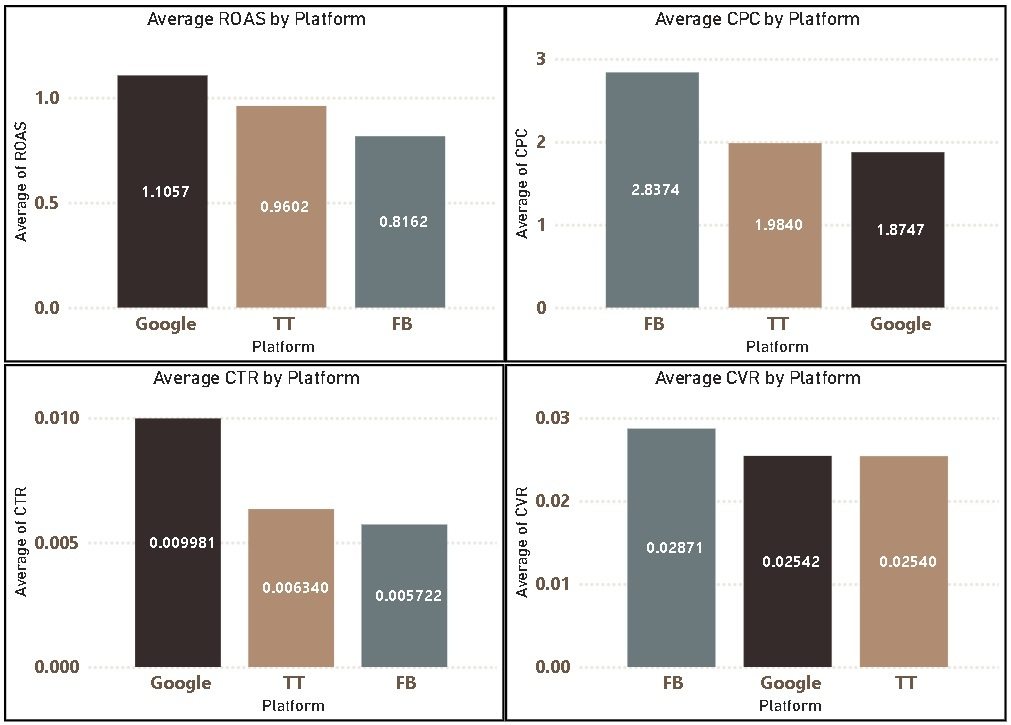
\includegraphics[width=1\textwidth]{images/metrics_by_platform.jpg}
	\caption{Performance Metrics by Platform}
	\label{fig:metrics_by_platform}
\end{figure}

\begin{itemize}
	\item FB exhibited the highest CVR out of all platforms which is offset by the high CPC and low CTR leading to its low ROAS.
	
	\item Google exhibited the highest CTR across platforms with the lowest Cost per Clicks.
	 
	\item From a business perspective, Google currently delivers the greatest overall value in contrast to FB platform based on their ROAS.
	
\end{itemize}

Drilling down on platforms by creative\_type we can see that Google search exhibited high ROAS while google Display exhibited one of the lowest ROAS as shown in Fig. \ref{fig:metrics_by_platform_creatives}. 

\begin{figure}[h]
	\centering
	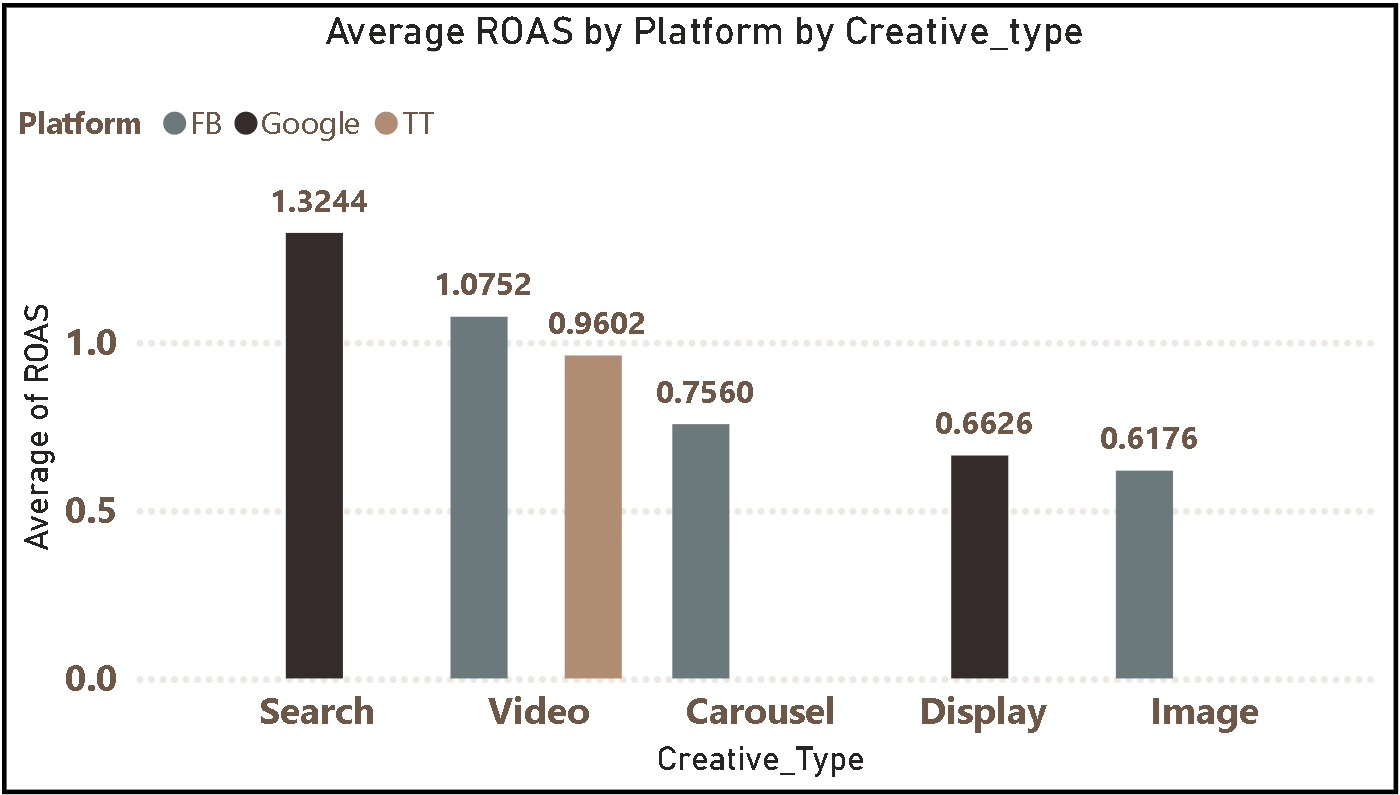
\includegraphics[width=0.6\textwidth]{images/ROAS_by_platform_by_creative.jpg}
	\caption{ROAS by Platform by Creative\_type}
	\label{fig:metrics_by_platform_creatives}
\end{figure}

This indicates that  \textbf{the performance of an ad campaign is not tied to the platform}, further analyses is required.
 
%%%%%%%%%%%%%%%%%%%%%%%%%%%%%%%%%%%%%%%%%%%%%%%%%%%%%%%%%%%%%%%%%%%%%%%%%%%%%%%%%%%%%%%%%%%%%%%%%%%%%%%%%%%%%%%%%%%%%%%%%%%%%%%%%%%%%%%%%%%%

\newpage
\section{Regional Performance Analysis}



\begin{figure}[h]
	\centering
	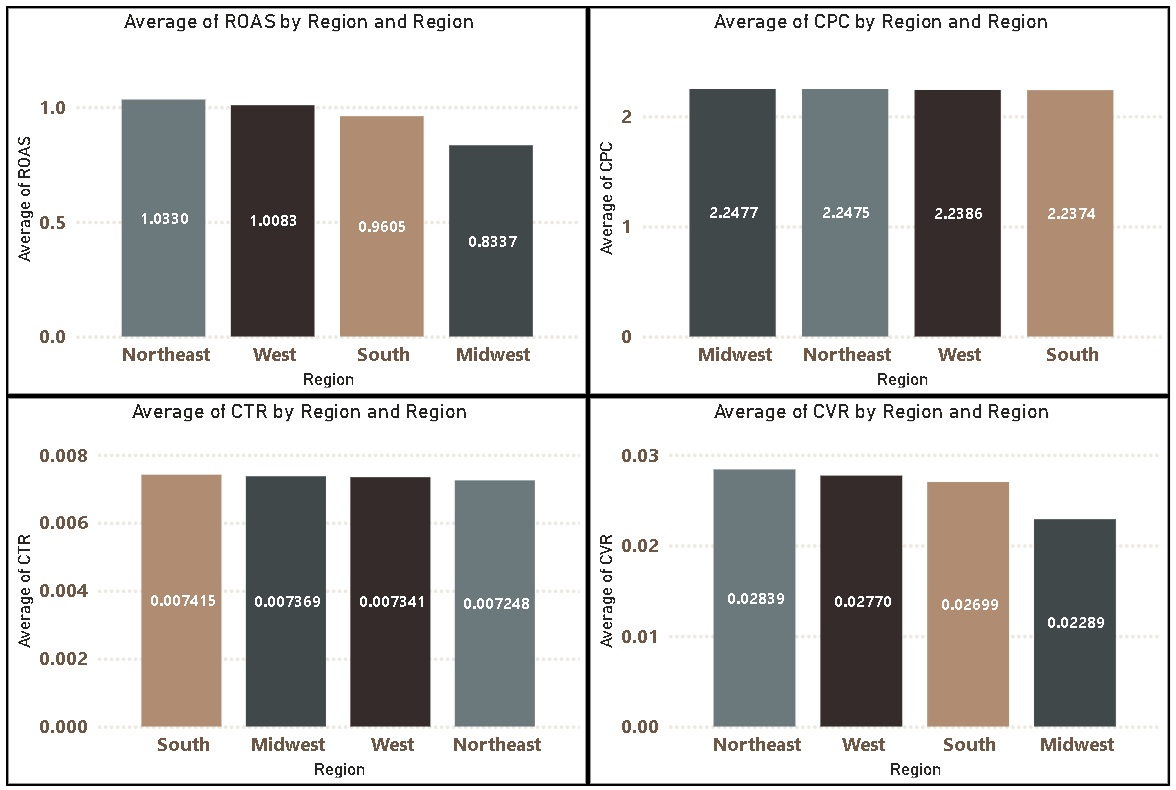
\includegraphics[width=0.8\textwidth]{images/metrics_by_region.jpg}
	\caption{Performance Metrics by Region}
	\label{fig:metrics_by_region}
\end{figure}



\begin{itemize}

	
	\item The \textbf{Midwest} consistently underperformed, recording both the lowest ROAS and the lowest conversion rate despite exhibiting click-through rates comparable to the other regions. This suggests that the primary challenge lies in converting interested users into customers rather than attracting engagement in this region.
	
	\item Because CTR and CPC did not differ significantly across regions, regional performance differences appear to be driven primarily by post-click behavior rather than differences in advertising cost or user engagement.
	

\end{itemize}




From a business perspective, further investigation should focus on \textbf{identifying factors that contribute to the Midwest's weaker conversion performance}. 

Potential explanations include regional differences in customer preferences, purchasing behavior, market competition, or campaign targeting strategies.


%%%%%%%%%%%%%%%%%%%%%%%%%%%%%%%%%%%%%%%%%%%%%%%%%%%%%%%%%%%%%%%%%%%%%%%%%%%%%%%%%%%%%%%%%%%%%%%%%%%%%%%%%%%%%%%%%%%%%%%%%%%%%%%%%%%%%%%%%%%%


\newpage
\section{Creative Performance Analysis}
Creative formats are highly imbalanced across campaigns, with certain creative types represented by only one or two campaigns as shown in Fig. \ref{fig:creative_type_count}. Consequently, comparisons should be interpreted as descriptive rather than causal.  

\begin{figure}[H]
	\centering
	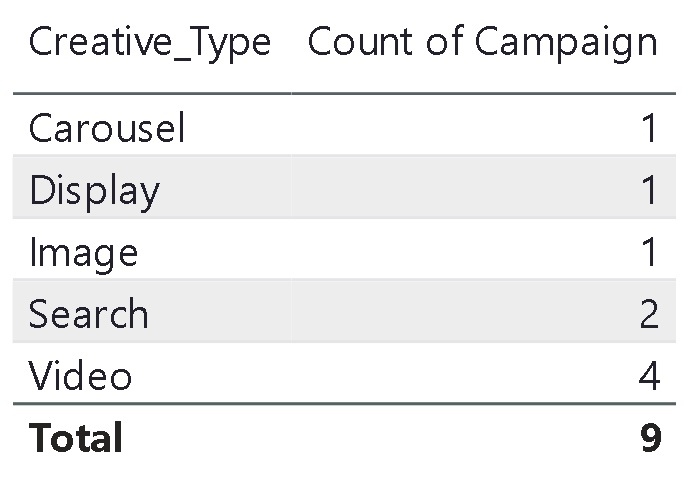
\includegraphics[width=0.3\textwidth]{images/creative_type_count.jpg}
	\caption{Creative Type Campaign counts}
	\label{fig:creative_type_count}
\end{figure}

Accordingly, the following observations are intended to describe aggregate performance patterns rather than isolate the causal effect of creative format. 

\begin{figure}[H]
	\centering
	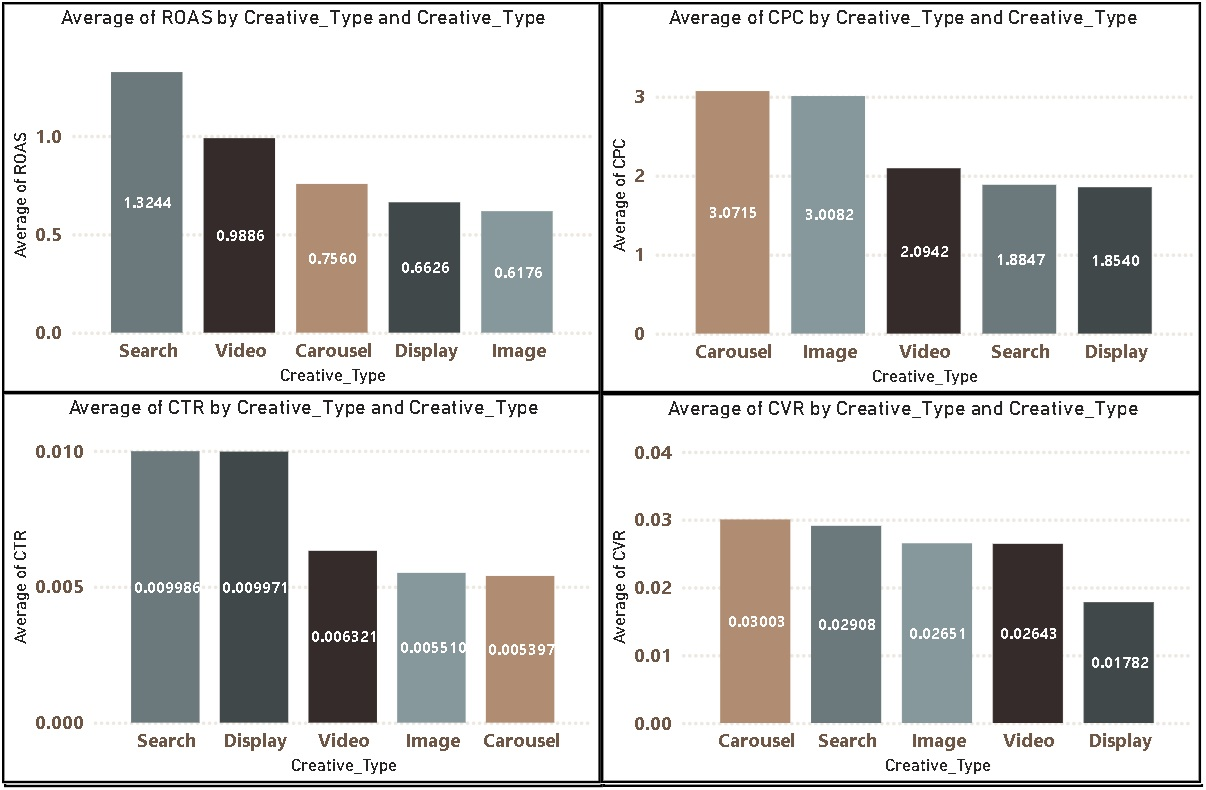
\includegraphics[width=0.8\textwidth]{images/metrics_by_creative.jpg}
	\caption{Performance Metrics by Creatives}
	\label{fig:metrics_by_creatives}
\end{figure}

Statistical significance tests for this section is shown in detail in Appendix \ref{appendix:creative_performance_analysis}. 
\begin{itemize}
	\item Search creatives exhibited the highest ROAS, whereas Display and Image exhibited the lowest ROAS.
	\item Search and Display successfuly generate clicks as shown by their CTR.
	\item In terms of traffic acquisition cost, carousel and image creatives are the most expensive.
	\item Carousel and Search exhibit the highest conversion efficiency as evidenced by their high CVR.
\end{itemize}

\subsection{Video Completion Rate vs Conversion}
We explored the relationship between video completion rate and conversion efficiency(CVR) as shown in Fig. \ref{fig:video_completion_rate}.


\begin{figure}[H]
	\centering
	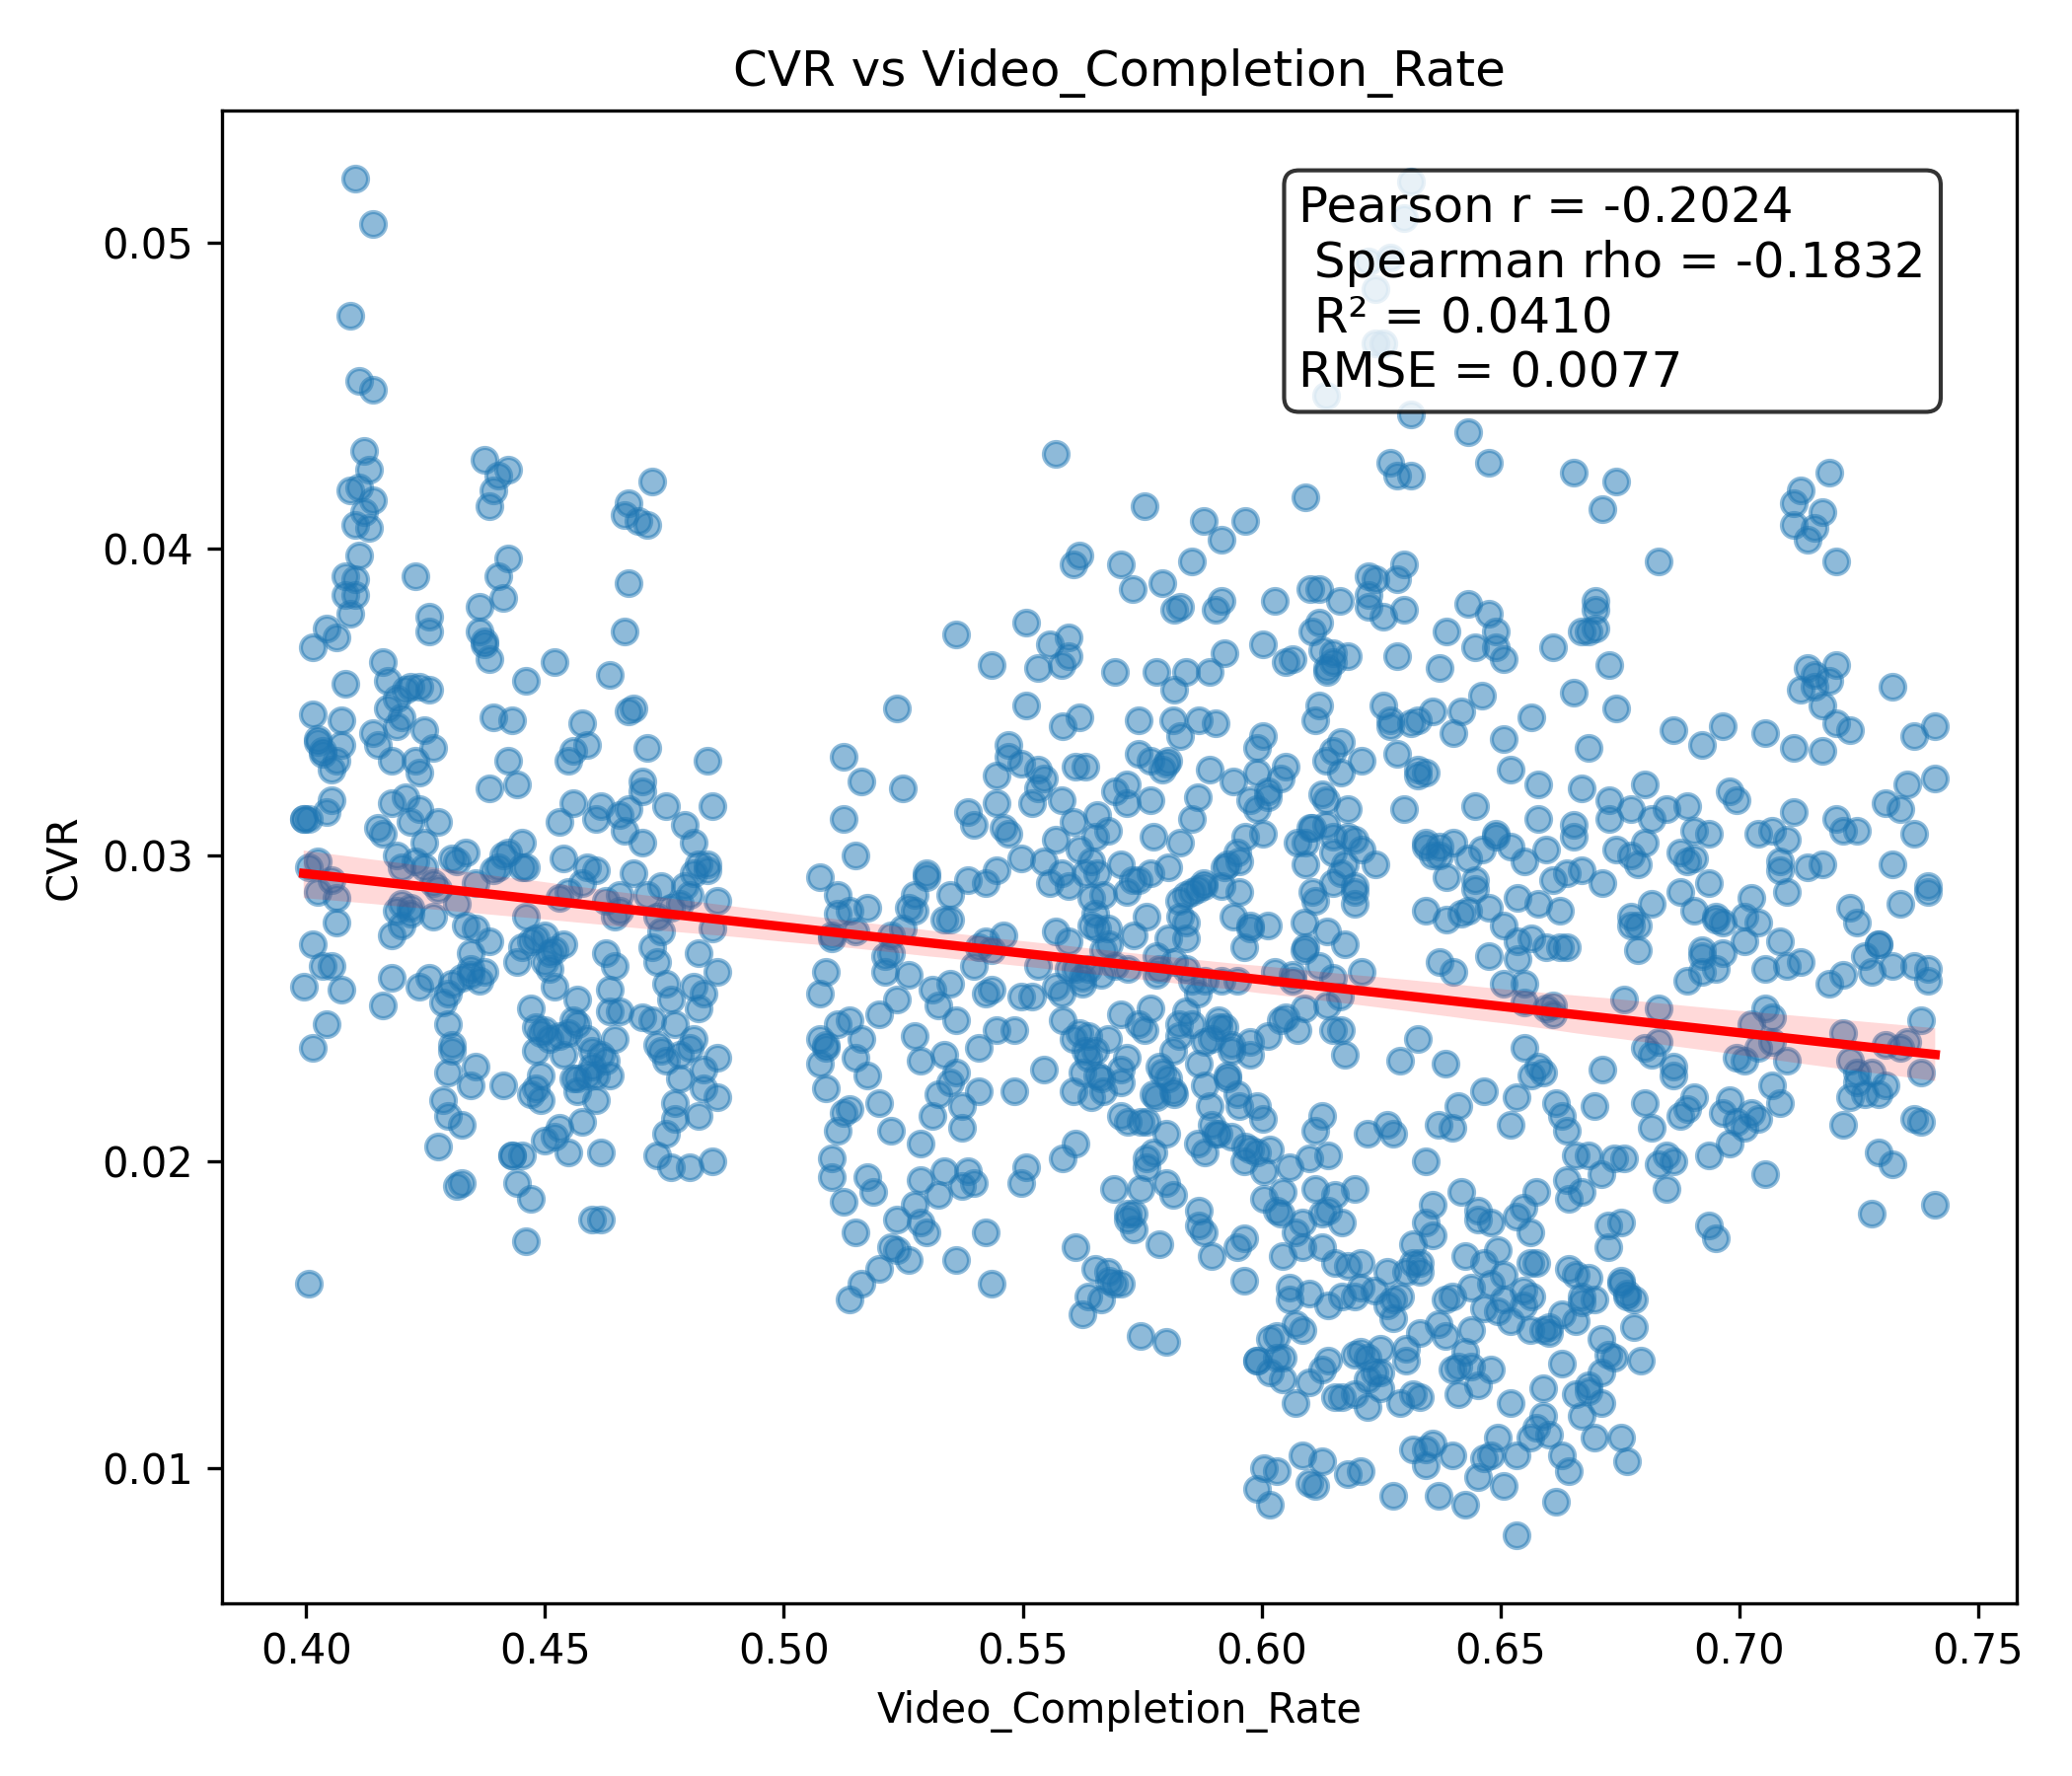
\includegraphics[width=0.7\textwidth]{images/CVR_vs_Video_Completion_Rate.png}
	\caption{CVR vs Video Completion Rate}
	\label{fig:video_completion_rate}
\end{figure}

There is no statistically significant correlation between the conversion rate(CVR) and video completion rate. 












	
	
	
%%%%%%%%%%%%%%%%%%%%%%%%%%%%%%%%%%%%%%%%%%%%%%%%%%%%%%%%%%%%%%%%%%%%%%%%%%%%%%%%%%%%%%%%%%%%%%%%%%%%%%%%%%%%%%%%%%%%%%
\section{Audience-Product Performance Analysis}
Performance of existing campaigns across different audience-product pairs was also investigated. 

\begin{figure}[H]
	\centering
	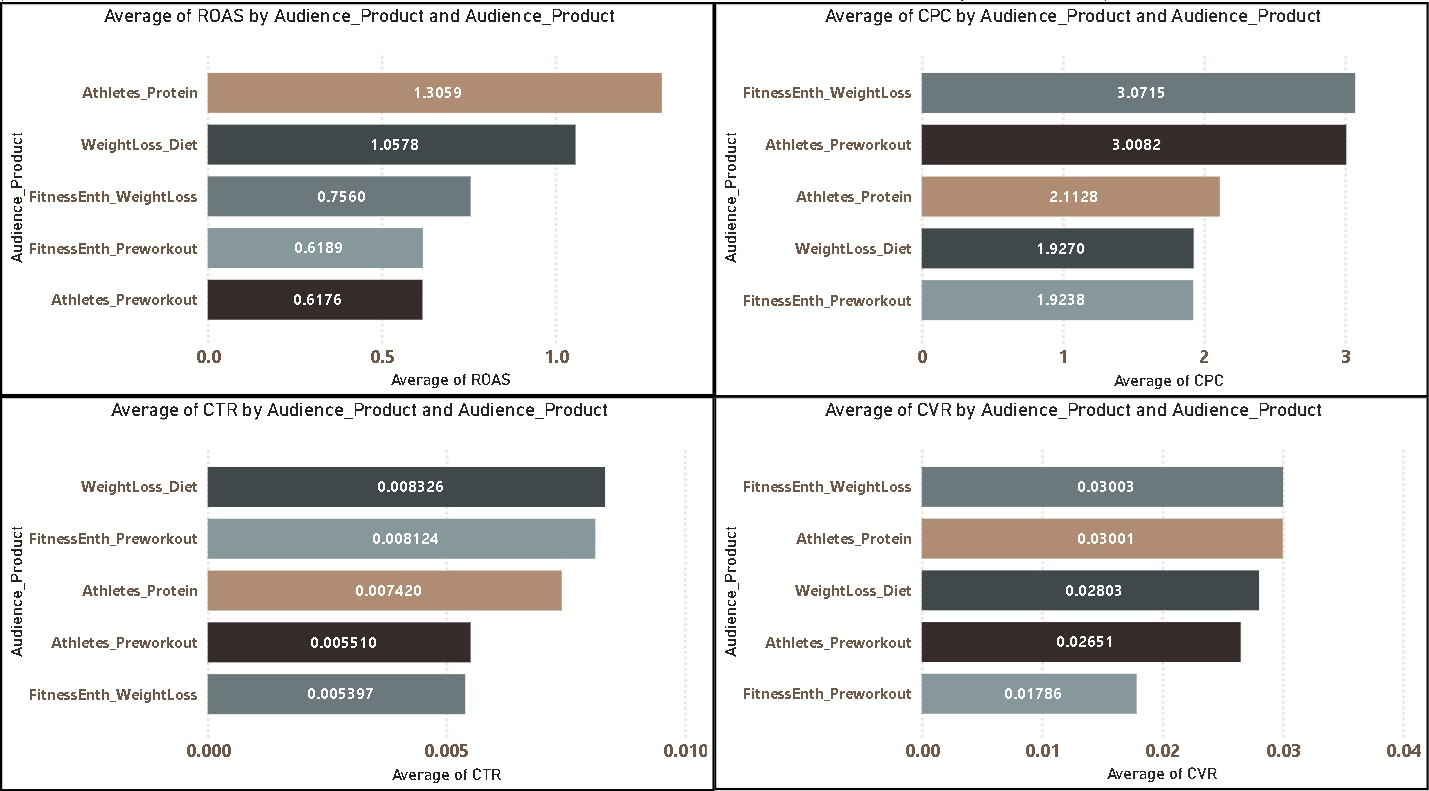
\includegraphics[width=1\textwidth]{images/metrics_by_audience-product.jpg}
	\caption{Performance Metrics by Audience-Product}
	\label{fig:audience-product}
\end{figure}

\begin{itemize}
	
	\item The \textbf{Athletes-Protein} combination demonstrated the strongest overall performance, achieving the highest ROAS while maintaining one of the highest conversion rates. This audience-product pairing appears to generate the greatest financial return from advertising investment.
	
	\item The \textbf{WeightLoss-Diet} combination also performed strongly, producing the second-highest ROAS, the highest click-through rate, and relatively low acquisition costs. These findings suggest that Diet campaigns are particularly effective when targeted toward individuals interested in weight loss.
	
	\item Both \textbf{Athletes-Preworkout} and \textbf{FitnessEnth-Preworkout} consistently exhibited poor ROAS despite differing levels of user engagement. This suggests that the weak financial performance of Pre-workout campaigns is not driven solely by audience selection, but may instead reflect broader issues related to the product offering, campaign messaging, pricing strategy, or post-click conversion experience.
	
	\item The \textbf{FitnessEnth-WeightLoss} combination achieved one of the highest conversion rates but also incurred the highest advertising cost per click. Although this audience converts effectively, its relatively high acquisition cost reduces overall profitability.
	
	\item Because statistically significant differences were observed across all four performance metrics, optimizing campaign performance should consider the \textbf{audience--product pairing} rather than treating audience and product category as independent marketing decisions.
	
\end{itemize}

From a business perspective, these findings suggest that future optimization efforts should evaluate the effectiveness of specific audience--product combinations rather than optimizing audience targeting or product campaigns independently. For example, investigating why the \textbf{WeightLoss--Diet} and \textbf{Athletes--Protein} pairings consistently outperform other combinations may reveal successful strategies that can be applied to other campaigns. Likewise, the consistently poor performance of both \textbf{Pre-workout} audience pairings suggests that improving audience selection alone is unlikely to substantially increase profitability. Instead, optimization should focus on the entire campaign strategy surrounding these pairings, including product positioning, promotional messaging, pricing, and landing page experience.


%%%%%%%%%%%%%%%%%%%%%%%%%%%%%%%%%%%%%%%%%%%%%%%%%%%%%%%%%%%%%%%%%%%%%%%%%%%%%%%%%%%%%%%%%%%%%%%%%%%%%%%%%%%%%%%%%%%%%%





%%%%%%%%%%%%%%%%%%%%%%%%%%%%%%%%%%%%%%%%%%%%%%%%%%%%%%%%%%%%%%%%%%%%%%%%%%%%%%%%%%%%%%%%%%%%%%%%%%%%%%%%%%%%%%%%%%%%%%

\section{Effect of Competitive Events}

The exploratory assessment examined whether campaign performance differed during periods with and without competitive events.

A complete summary of the statistical analyses, including assumption checks, Kruskal--Wallis tests, and pairwise comparisons, is provided in Appendix~\ref{appendix:competitive_event_performance_analysis}.

\begin{figure}[h]
	\centering
	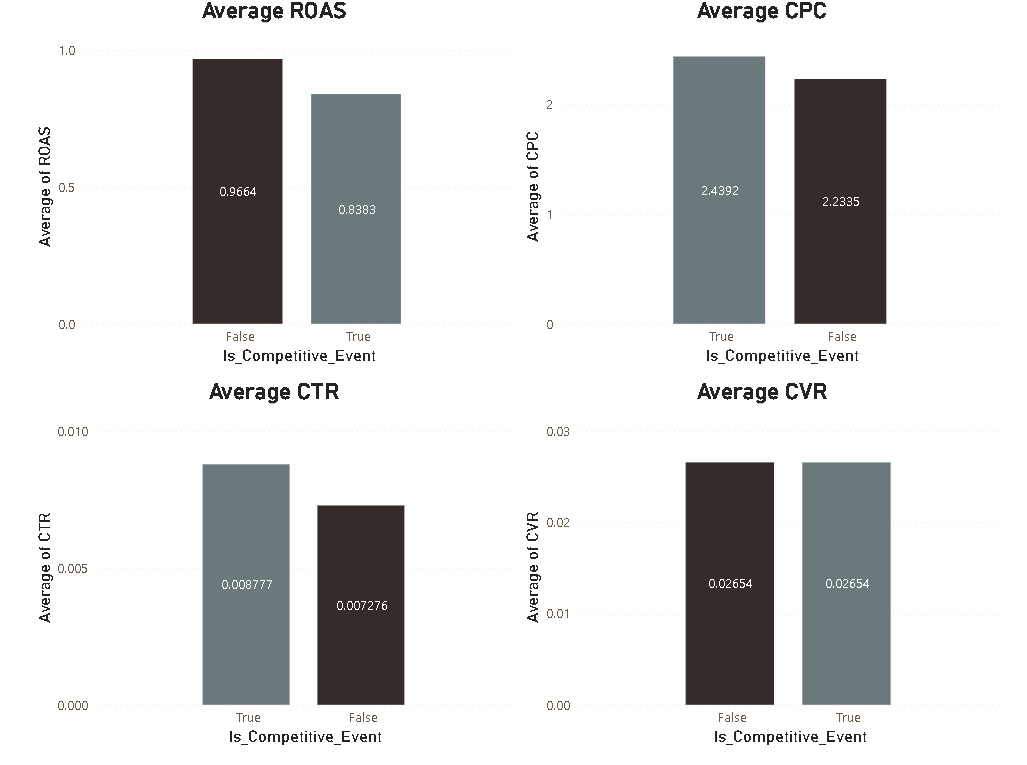
\includegraphics[width=\textwidth]{images/competitive_event_effect.jpg}
	\caption{Comparison of campaign performance during competitive and non-competitive periods.}
	\label{fig:competitive_event_summary}
\end{figure}

Figure~\ref{fig:competitive_event_summary} summarizes the influence of competitive events on the four primary advertising performance metrics.

Campaigns conducted during competitive events achieved a significantly lower average ROAS (0.838) than campaigns conducted outside competitive periods (0.966), indicating reduced advertising profitability (Appendix~\ref{appendix:competitive_event_performance_analysis_ROAS}).

Interestingly, campaigns during competitive events generated significantly higher CTR (0.88\% versus 0.73\%), suggesting that advertisements attracted greater user engagement despite increased market competition (Appendix~\ref{appendix:competitive_event_performance_analysis_CTR}).

However, this increase in engagement did not translate into improved purchasing behavior. Conversion rates remained statistically unchanged between competitive and non-competitive periods (approximately 2.65\%), indicating that users who clicked advertisements were equally likely to complete a purchase regardless of competitive conditions (Appendix~\ref{appendix:competitive_event_performance_analysis_CVR}).

Competitive events were also associated with significantly higher CPC (\$2.44 versus \$2.23), indicating that advertisers paid more to acquire each click (Appendix~\ref{appendix:competitive_event_performance_analysis_CPC}).

Taken together, these findings suggest that competitive events primarily reduce campaign profitability by increasing advertising costs rather than by reducing customer purchase intent. Although advertisements attracted more clicks during competitive periods, the higher acquisition cost combined with unchanged conversion performance resulted in significantly lower ROAS.

From a business perspective, campaigns scheduled during competitive periods may require stronger creative assets, more precise audience targeting, or more compelling promotional offers to justify the higher advertising costs. Alternatively, campaigns focused primarily on maximizing profitability may benefit from allocating a larger portion of the advertising budget to less competitive periods where comparable conversion rates can be achieved at lower acquisition costs.


\section{Temporal Analysis}




\appendix
\renewcommand{\chaptername}{Appendix}

\clearpage
\singlespacing


\addcontentsline{toc}{chapter}{Appendices}

\chapter{Data Quality and Initial Exploratory Assessment}\label{appendix:data_quality}
	
\section{Data Quality Assessment}

Prior to conducting business intelligence analysis, the advertising campaign dataset was evaluated to ensure its quality, reliability, and suitability for analysis. The objective of this assessment is to identify potential data quality issues, validate the performance metrics used throughout the project, examine unusual observations, and establish a set of baseline metrics that will guide subsequent business analysis.

The dataset contains daily advertising campaign performance across multiple platforms, regions, target audiences, product categories, and creative types during the first quarter of 2024.
	
	
	
	
\subsection{Data Type}

The data types of all variables were first examined to verify that each column was stored using an appropriate data type. As shown in\textit{ Fig. \ref{fig:check_datatype}}, numerical variables were stored as either \texttt{int64} or \texttt{float64}, categorical variables as \texttt{object}, the \texttt{Date} column as \texttt{datetime64[ns]}, and the \texttt{Is\_Competitive\_Event} variable as a boolean. 

\begin{figure}[h]
	\centering
	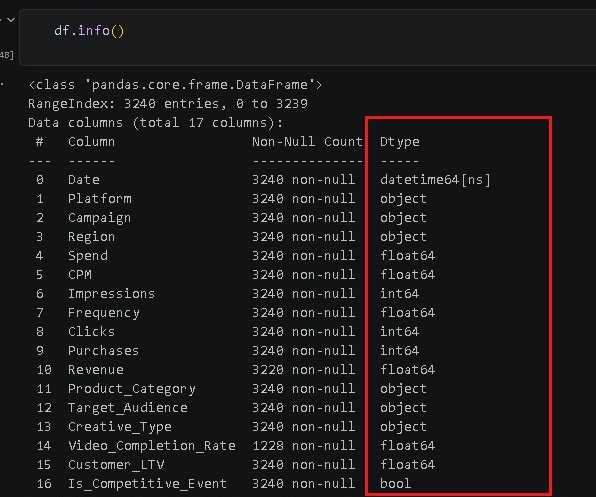
\includegraphics[width=0.45\textwidth]{images/check_datatype.jpg}
	\caption{Checking datatypes of the dataframe}
	\label{fig:check_datatype}
\end{figure}
No inconsistencies in data types were identified; therefore, no type conversions were required.

\subsection{Duplicate Records}

The dataset was examined for duplicate observations.

\begin{figure}[h]
	\centering
	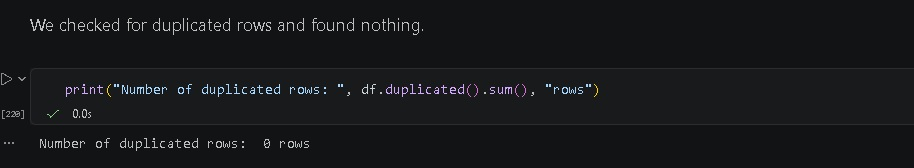
\includegraphics[width=0.8\textwidth]{images/duplicate_records.jpg}
	\caption{Checking for duplicate records}
	\label{fig:duplicate_records}
\end{figure}


No duplicate records were identified as shown in \textit{Fig. \ref{fig:duplicate_records}}.



\subsection{Data Completeness}

The dataset was examined for missing values to determine whether incomplete observations could affect subsequent analyses.

\begin{itemize}
	
	\item \textbf{Revenue}
	
	A sample of these datapoints are shown in \textit{Fig. \ref{fig:missing_values}}. It can be seen that twenty observations (approximately 0.6\% of the dataset) contained missing revenue values.
	\begin{figure}[h]
		\centering
		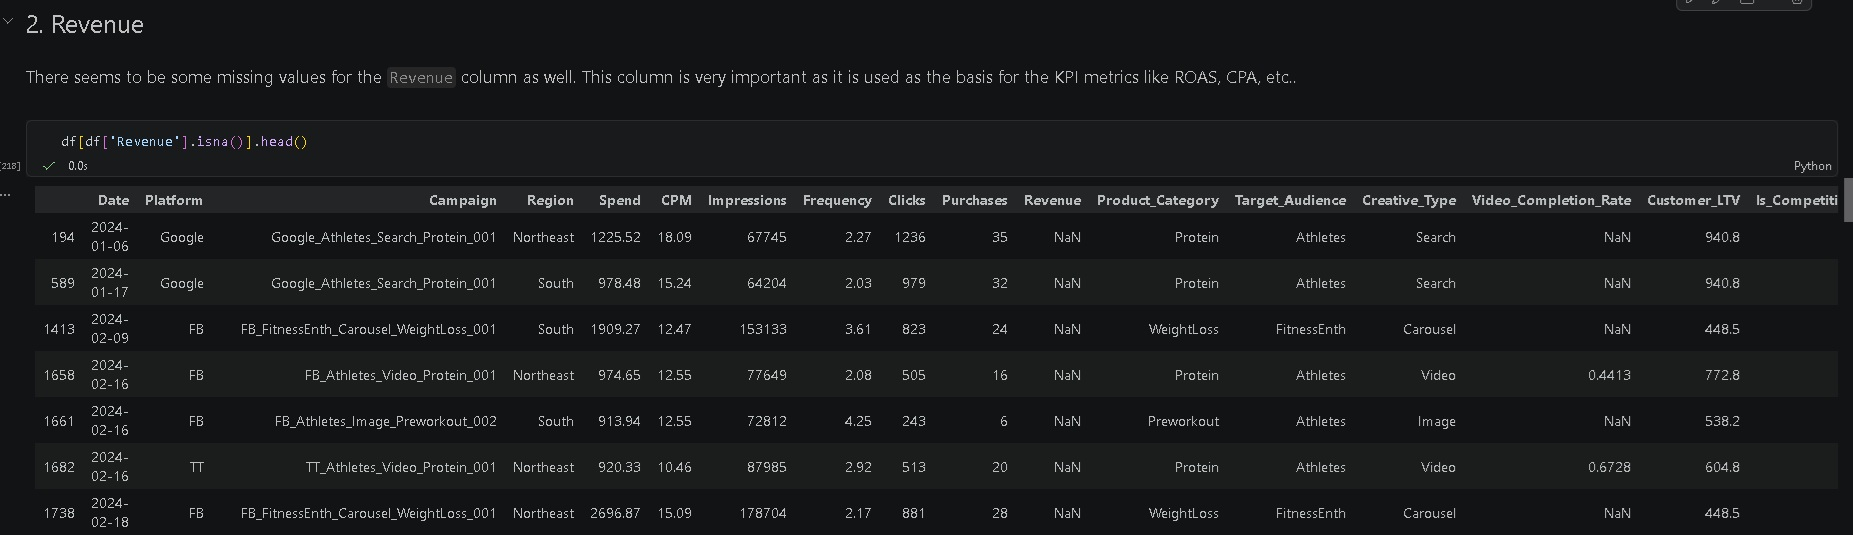
\includegraphics[width=1\textwidth]{images/revenue_missing_values.jpg}
		\caption{Sample datapoints with missing revenues.}
		\label{fig:missing_values}
	\end{figure}



	
	Because these represented a very small proportion of the data and no systematic pattern of missingness was identified, the corresponding observations were removed as shown in\textit{ Fig. \ref{fig:drop_missing_values}} prior to analysis.
\begin{figure}[h]
	\centering
	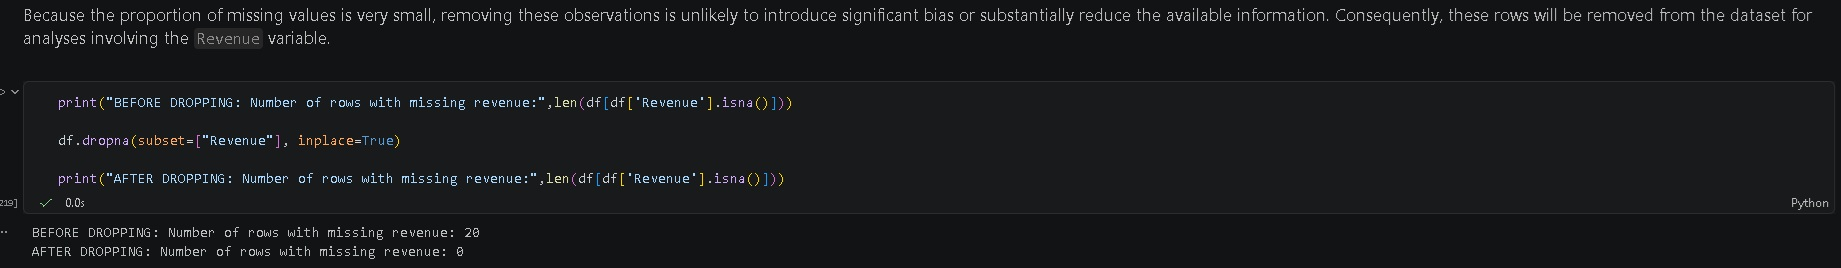
\includegraphics[width=1\textwidth]{images/drop_missing_revenue.jpg}
	\caption{Dropped datapoints with missing revenues.}
	\label{fig:drop_missing_values}
\end{figure}
		
	
	\item \textbf{Video Completion Rate}
	
	A large number of missing values were initially observed in the \textit{Video Completion Rate} variable. Around 62\% of the total dataset! 
	
\begin{figure}[h]
	\centering
	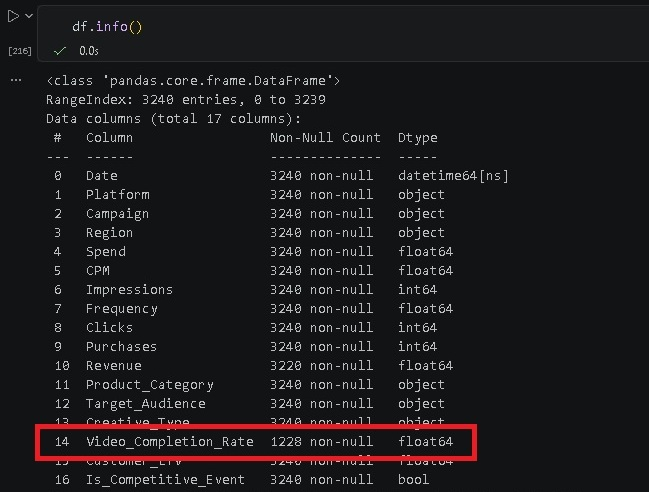
\includegraphics[width=0.45\textwidth]{images/video_completion_missing.jpg}
	\caption{\texttt{video\_completion\_rate} missing values}
	\label{fig:video_completion_missing}
\end{figure}
	
	
	
	
	Further investigation revealed that this metric is only applicable to \textbf{campaigns using video advertisements}. After restricting the dataframe to video creatives, \textbf{only 212 missing observations remained} as shown in \textit{Fig. \ref{fig:filtered_video_completion_missing}}. 
	
\begin{figure}[h]
	\centering
	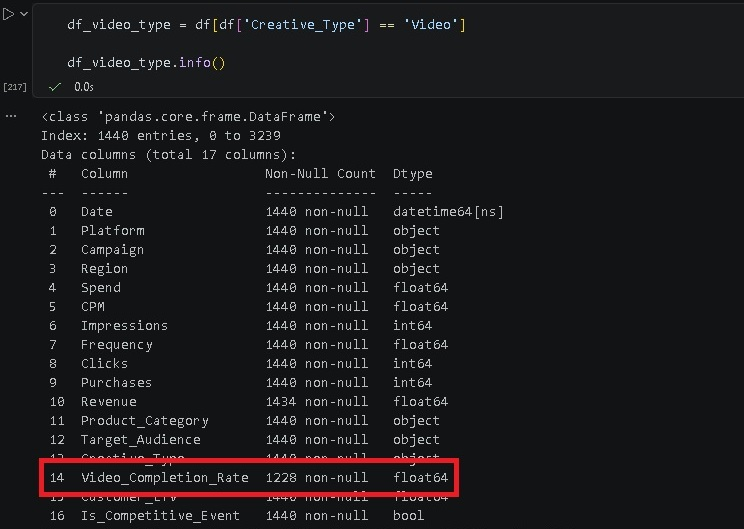
\includegraphics[width=0.45\textwidth]{images/filtered_video_completion_missing.jpg}
	\caption{DataFrame filtered to video creative types}
	\label{fig:filtered_video_completion_missing}
\end{figure}	
	

	Consequently, these missing values were treated as \textbf{structurally missing} rather than data quality issues, and analyses involving this variable will use only the relevant subset of campaigns.
	
\end{itemize}

	\subsection{Logical Consistency Checks}
	
	Several validation checks were performed to identify logically inconsistent observations.
	
	\subsubsection{0 Clicks with non-zero purchase}
	
	I noticed that there were rows with 0 clicks but has non-zero Purchases, which I thought was weird at first. How are they able to purchase without clicking the ad. 
	
	Apparently, this happens in real world scenarios and they are called \textbf{view-through conversions}. People see the ad, they don't click it then later that evening, they remembered the brand and typed the website into google and bought the product.
	
	\begin{figure}[h]
		\centering
		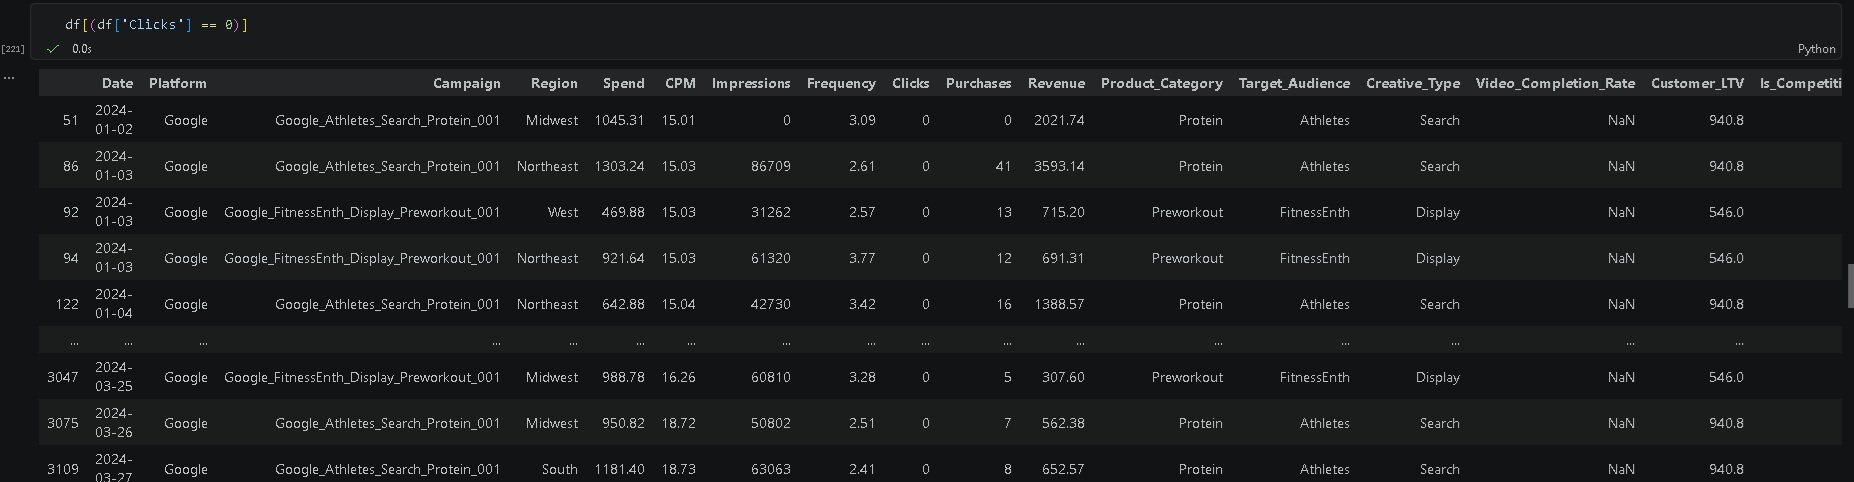
\includegraphics[width=0.8\textwidth]{images/0clicks_non0purchase.jpg}
		\caption{Sample datapoints with 0 clicks but non-zero purchase}
		\label{fig:0clicks_non0purchase}
	\end{figure}
	
	
	But, at this point, I was wondering how they know which ad actually influenced the purchased without click or what if the buyer interacted with multiple ads before purchasing(cross-channel conversions). Apparently, this is related to \textbf{attribution}, and there are multiple attribution models like \textbf{last\_click attribution}, \textbf{first-click attribution}, \textbf{linear\_attribution}, etc.. which is not part of this data cleaning process. 
	
	So, for now, I'll just assume that this dataset was collected using a certain attribution model and leave it at that. This justifies the 0 clicks with non-zero purchase.
	
\begin{tcolorbox}
	\textbf{Side Note:} After the data cleaning, all rows with zero clicks belong to the Google platform. (For the time being, this is just an observation. I'm noting it here so I don't forget to investigate it later.)
\end{tcolorbox}
	
	\subsubsection{0 Impressions with non-zero Cost-Per-Mile(CPM)}
	
	Cost Per Mille (CPM) measures the advertising cost required to generate 1,000 impressions and is commonly used to evaluate the cost efficiency of awareness campaigns.
	
	\begin{equation}
		\text{CPM} = \frac{\text{Spend}}{\text{Impressions}} \times 1000
	\end{equation}
	
	Because impressions appear in the denominator, CPM is undefined when the number of impressions is zero.
	
	During the data quality assessment, 47 observations (approximately 1.45\% of the dataset) were identified with \texttt{Impressions = 0} but non-zero with CPM values. 
	

	Furthermore, all of these observations originated from the Midwest region as shown in \textit{Fig. \ref{fig:0impression}}, suggesting a systematic reporting inconsistency rather than isolated data entry errors.
	
	\begin{figure}[h]
		\centering
		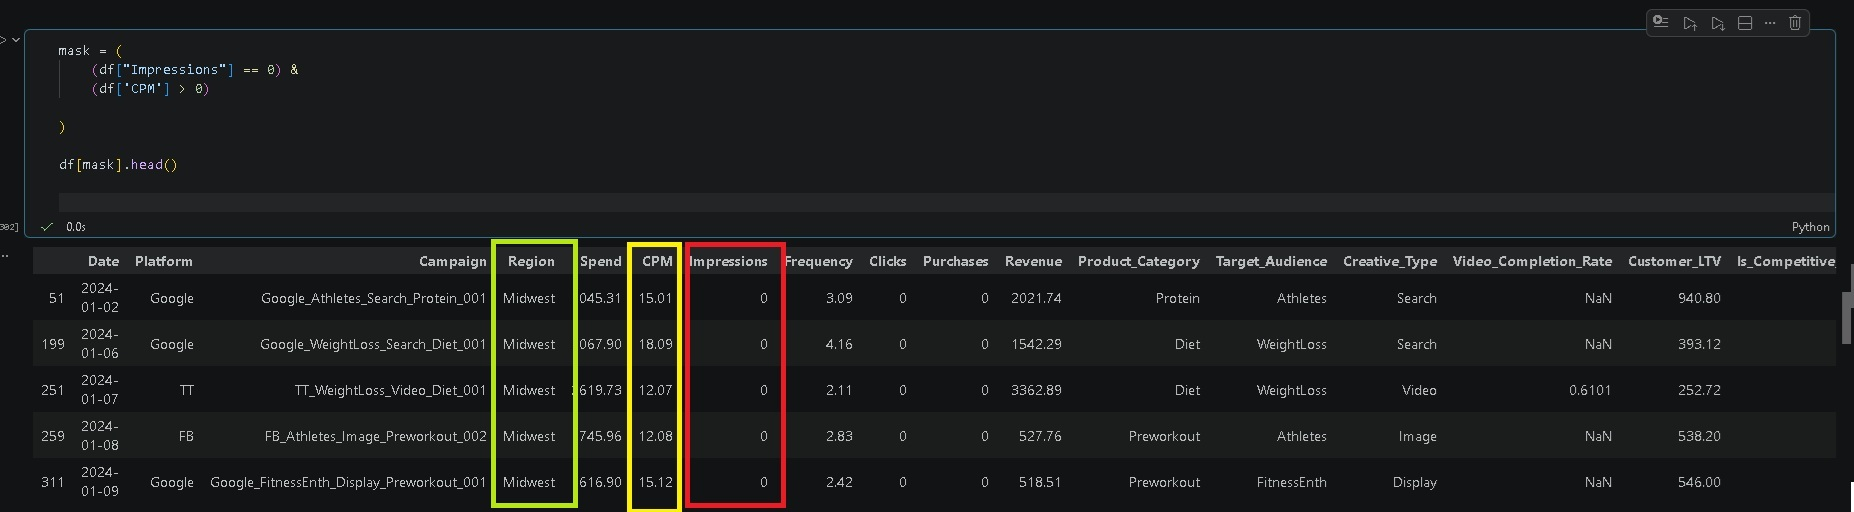
\includegraphics[width=0.8\textwidth]{images/0impressions.jpg}
		\caption{Sample rows that has 0 impressions with non-zero CPM}
		\label{fig:0impression}
	\end{figure}
	
	
	Since these observations violate the definition of CPM and the 0 impressions value could affect the calculation of other performance metrics, such as CTR and CVR, they were removed from the dataset prior to analysis.
	
	\begin{figure}[h]
		\centering
		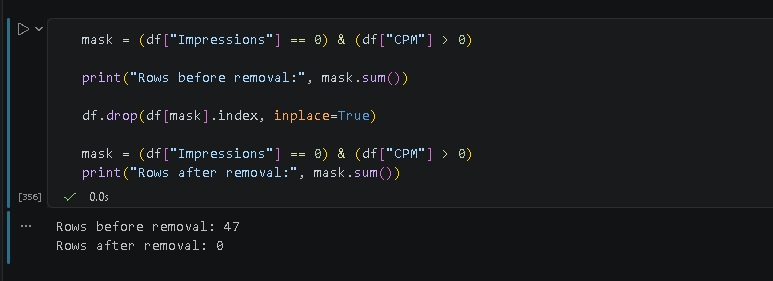
\includegraphics[width=0.8\textwidth]{images/0impressionscount.jpg}
		\caption{Dropped Rows that has 0 impressions with non-zero CPM}
		\label{fig:0impression_count}
	\end{figure}
	
		\subsection{Outlier Assessment}
	Boxplots were used to identify potential outliers across the numerical variables as shown in \textit{Fig. \ref{fig:box_plots}}. Severe outliers were identified for the Spend column and will be investigated in this section.
	\begin{figure}[h]
		\centering
		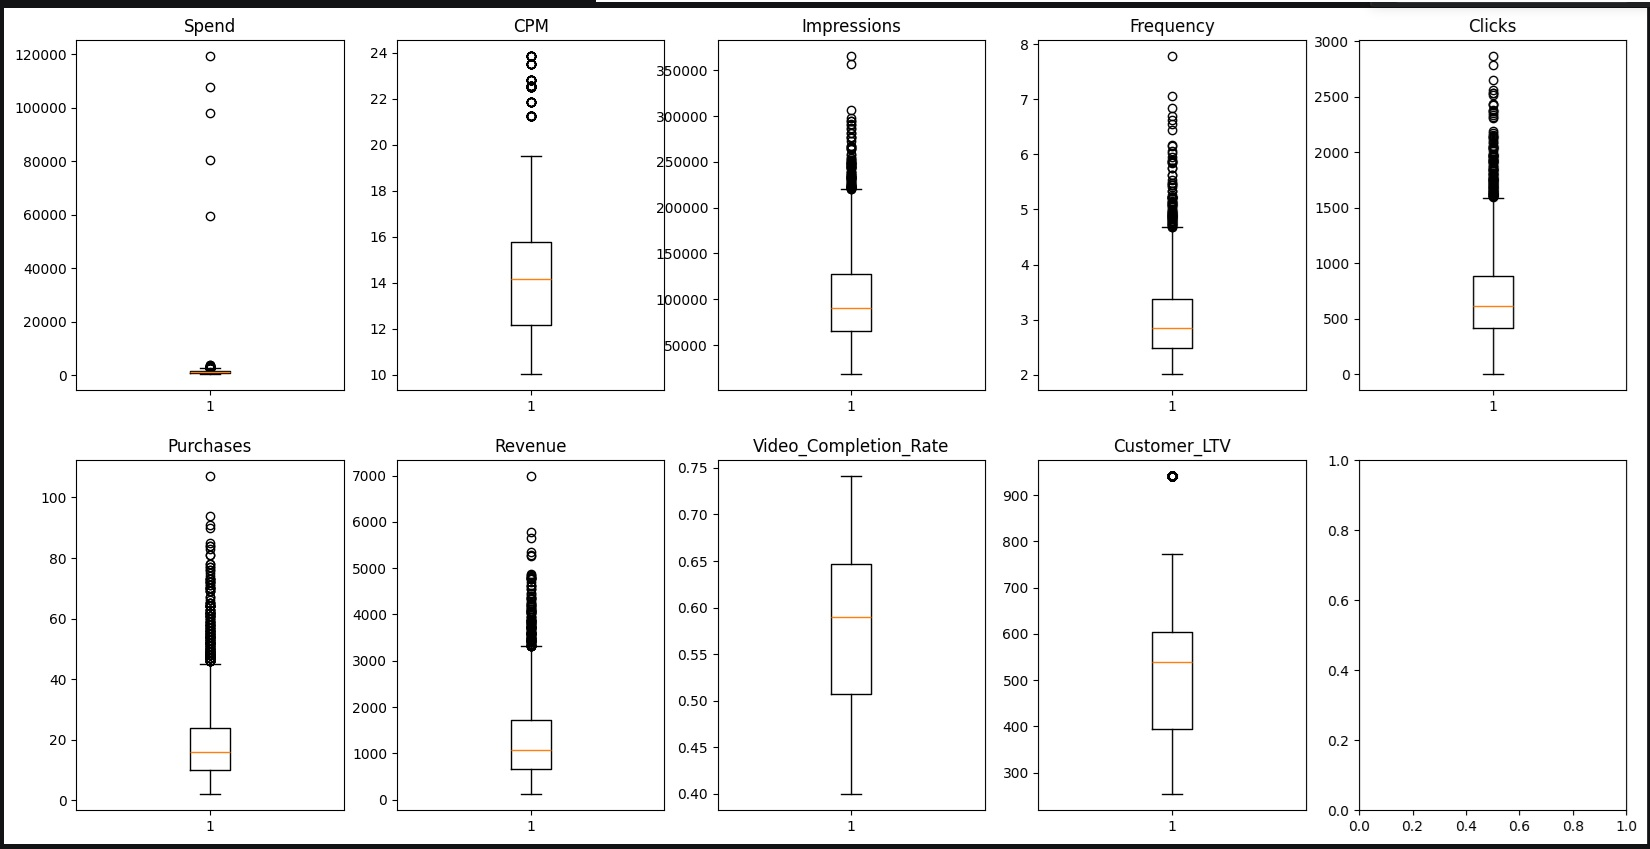
\includegraphics[width=1\textwidth]{images/box_plotsjpg.jpg}
		\caption{Boxplots for all numerical columns of the dataframe}
		\label{fig:box_plots}
	\end{figure}
	
	
	\subsubsection{\texttt{Spend} severe outliers investigation}
	First, I listed the 5 datapoints with severe \texttt{Spend} outliers as shown in \textit{Fig. \ref{fig:spend_outliers}}. I noticed that in this 5 datapoints, the \textbf{CPM do not match the Ad Spend and Impression}. This tells me that there is a possibility that there are more rows with mismatched CPM. 
	
\begin{figure}[h]
	\centering
	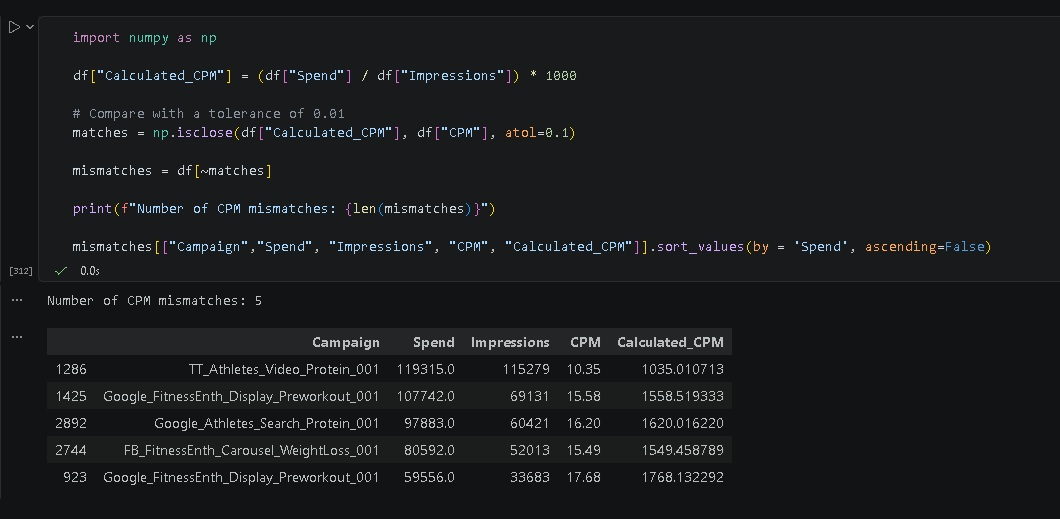
\includegraphics[width=1\textwidth]{images/CPM_mismatch_list.jpg}
	\caption{Number of rows with CPM mismatch}
	\label{fig:CPM_mismatch_list}
\end{figure}	
	
	So, I checked and found out that only these 5 rows have mismatched CPM as shown in \textit{Fig. \ref{fig:CPM_mismatch_list}}, after dropping the rows from earlier(the ones with 0 impression,clicks and purchases).
	
	\begin{figure}[h]
		\centering
		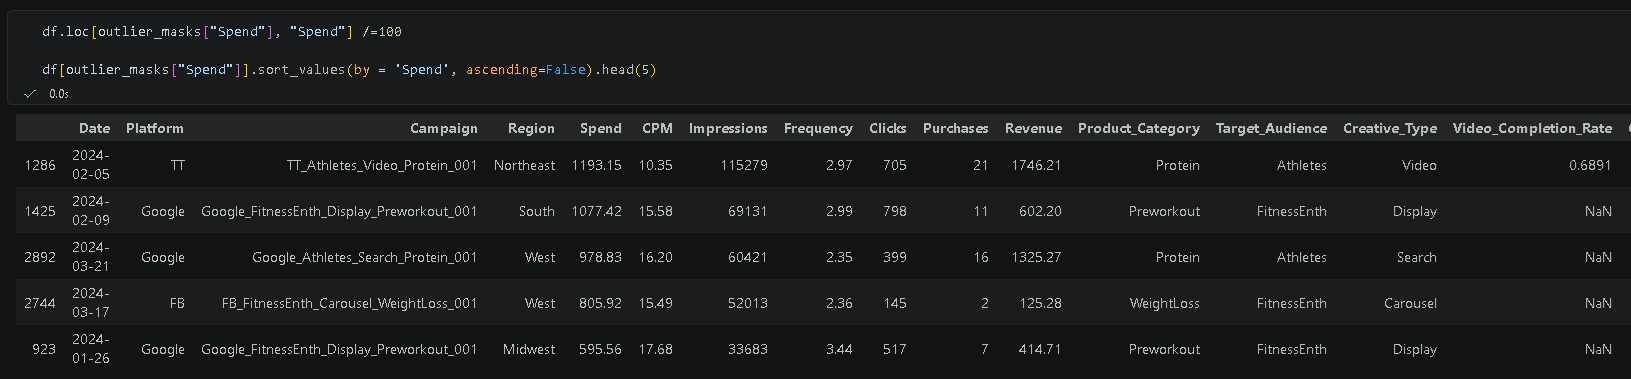
\includegraphics[width=1\textwidth]{images/severe_spend_outlier_list.jpg}
		\caption{Datapoints with severe \texttt{Spend} outliers}
		\label{fig:spend_outliers}
	\end{figure}
	
	Then, I plotted the \texttt{Spend} boxplots of these Campaign Ads.
	
	\begin{figure}[h]
		\centering
		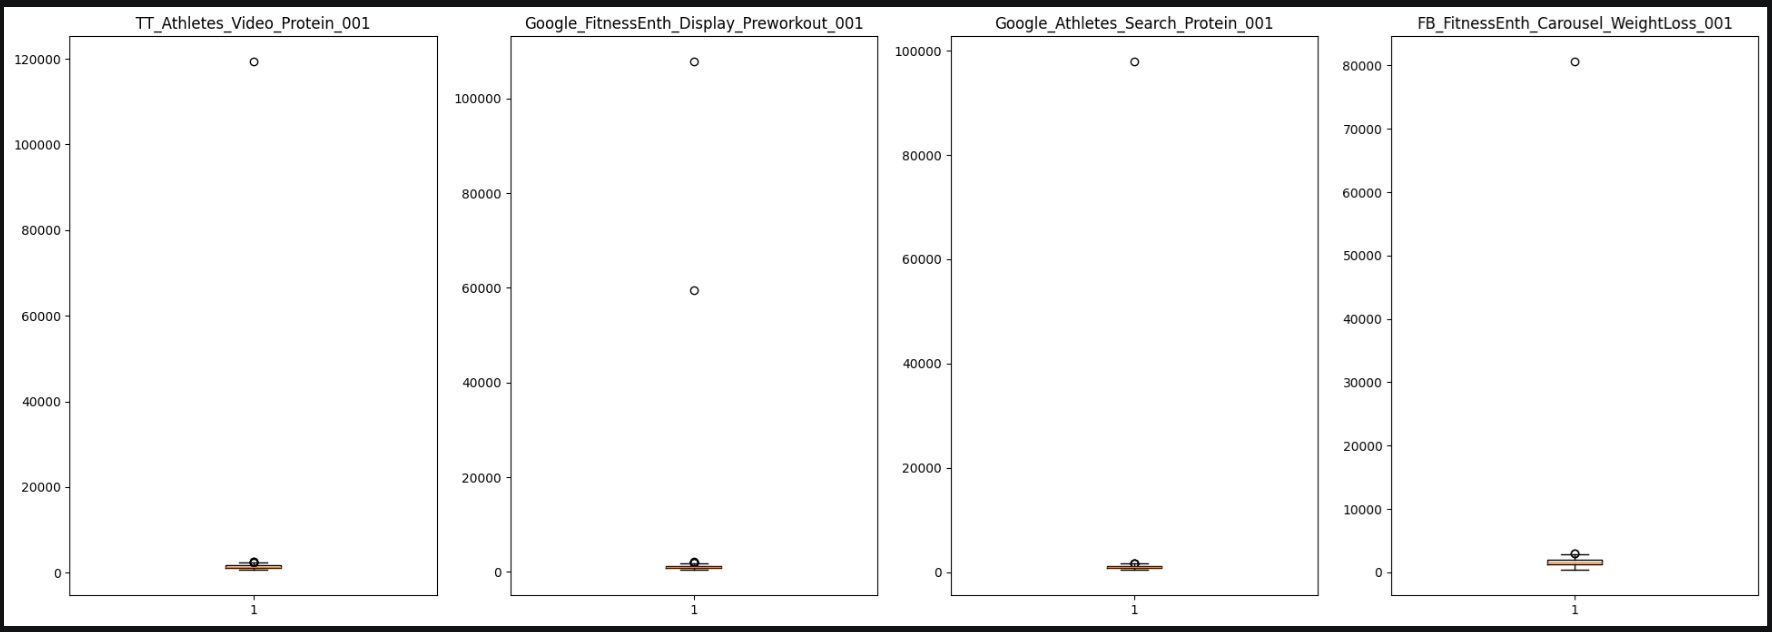
\includegraphics[width=1\textwidth]{images/severe_spend_outlier_boxplot.jpg}
		\caption{\texttt{Spend} boxplots for campaign ads with severe \texttt{Spend} outliers}
		\label{fig:spend_outliers_boxplot}
	\end{figure}
	
	
	From this analysis, I noticed the following consistencies:
	\begin{enumerate}
		\item The reported CPM values(from datapoints with severe \texttt{Spend} outliers) were exactly one-hundredth of the values calculated from the corresponding Spend and Impressions.
		\item The calculated CPM values do not match the `Impressions` and `Spend` columns, and this is limited only to the 5 reported rows with severe `Spend` outliers.
		
		\item Inspection of the affected campaigns showed that the unusually large Spend values occurred only on a single day and were not associated with competitive events.
		
	\end{enumerate}
	Since the discrepancy was systematic (a factor of 100) and limited to these five observations, the Spend values were divided by 100 to restore consistency with the reported CPM values.
	

	
	\subsection{Data Cleaning Summary}
	
	The data cleaning process consisted of:
	
	\begin{itemize}
		\item Verified variable data types
		
		\item Verifying duplicate observations
		
		\item Removing observations(20 datapoints) with missing revenue.
		
		\item Retaining structurally missing Video Completion Rate values.
		
		\item Retaining valid view-through conversions.
		
		\item Removing observations(47 datapoints) with 0 clicks,impressions and purchases with non-zero purchase. 
		
		\item Addressed severe \texttt{Spend} outliers.
		

	
		
	\end{itemize}
	
	Overall, the dataset was determined to be sufficiently complete and reliable for subsequent analysis.
	


\chapter{Statistical Test Results of Metrics across Platforms}


This appendix presents the complete statistical test results supporting the analyses discussed in the main report.

\section{Platform Performance Analysis}\label{appendix:platform_performance_analysis}

\subsection{Return on Advertising Spend (ROAS)}\label{appendix:platform_performance_analysis_ROAS}

\subsubsection{Descriptive Statistics}

\begin{table}[H]
	\centering
	\caption{Descriptive statistics for ROAS by platform.}
	\begin{tabular}{lcccc}
		\toprule
		Platform & Mean & Median & Std. Dev. & Count \\
		\midrule
		Facebook & 0.8162 & 0.7499 & 0.4225 & 1054 \\
		Google   & 1.1057 & 0.9456 & 0.6495 & 1053 \\
		TikTok   & 0.9602 & 0.8625 & 0.4950 & 1066 \\
		\bottomrule
	\end{tabular}
\end{table}

\subsubsection{Assumption Tests}

\subsubsection{Shapiro--Wilk Test}

\begin{table}[H]
	\centering
	\begin{tabular}{lc}
		\toprule
		Platform & p-value \\
		\midrule
		Facebook & $<0.0001$ \\
		Google & $<0.0001$ \\
		TikTok & $<0.0001$ \\
		\bottomrule
	\end{tabular}
\end{table}

All platform distributions significantly deviated from normality ($p<0.05$).

\vspace{0.3cm}

\subsubsection{Levene's Test}

\begin{table}[H]
	\centering
	\begin{tabular}{lc}
		\toprule
		Statistic & Value \\
		\midrule
		p-value & $<0.0001$ \\
		\bottomrule
	\end{tabular}
\end{table}

The variability of \textbf{ROAS differed significantly} across platforms.

\vspace{0.3cm}

\subsubsection{Kruskal--Wallis Test}

\begin{table}[H]
	\centering
	\begin{tabular}{lcc}
		\toprule
		Statistic & Value \\
		\midrule
		H-statistic & 106.6989 \\
		p-value & $<0.0001$ \\
		\bottomrule
	\end{tabular}
\end{table}

The Kruskal--Wallis test indicates statistically significant differences in ROAS across advertising platforms.

\vspace{0.3cm}

\subsubsection{Dunn Post-hoc Test}

\begin{table}[H]
	\centering
	\caption{Pairwise Dunn test p-values (Bonferroni adjusted).}
	\begin{tabular}{lccc}
		\toprule
		& Facebook & Google & TikTok \\
		\midrule
		Facebook & -- & $<0.0001$ & $<0.0001$ \\
		Google & $<0.0001$ & -- & 0.0002 \\
		TikTok & $<0.0001$ & 0.0002 & -- \\
		\bottomrule
	\end{tabular}
\end{table}

\subsubsection{Summary}
\begin{itemize}
	\item The highest average ROAS was achieved by Google (1.1057).
	\item The lowest average ROAS was observed for FB (0.8162).
	\item Differences of ROAS between platforms are statistically significant ($p<0.05$).
\end{itemize}

\subsection{Click-Through Rate (CTR)} \label{appendix:platform_performance_analysis_CTR}

\subsubsection{Descriptive Statistics}

\begin{table}[H]
	\centering
	\caption{Descriptive statistics for CTR by platform.}
	\begin{tabular}{lcccc}
		\toprule
		Platform & Mean & Median & Std. Dev. & Count \\
		\midrule
		Facebook & 0.0057 & 0.0056 & 0.0021 & 1054 \\
		Google   & 0.0100 & 0.0098 & 0.0052 & 1053 \\
		TikTok   & 0.0063 & 0.0062 & 0.0018 & 1066 \\
		\bottomrule
	\end{tabular}
\end{table}

\subsubsection{Assumption Tests}

\subsubsection{Shapiro--Wilk Test}

\begin{table}[H]
	\centering
	\begin{tabular}{lc}
		\toprule
		Platform & p-value \\
		\midrule
		Facebook & $<0.0001$ \\
		Google & $<0.0001$ \\
		TikTok & $<0.0001$ \\
		\bottomrule
	\end{tabular}
\end{table}

All platform distributions significantly deviated from normality ($p<0.05$).

\vspace{0.3cm}

\subsubsection{Levene's Test}

\begin{table}[H]
	\centering
	\begin{tabular}{lc}
		\toprule
		Statistic & Value \\
		\midrule
		p-value & $<0.0001$ \\
		\bottomrule
	\end{tabular}
\end{table}

The variability of CTR\textbf{ differed significantly across platforms}.

\vspace{0.3cm}

\subsubsection{Kruskal--Wallis Test}

\begin{table}[H]
	\centering
	\begin{tabular}{lc}
		\toprule
		Statistic & Value \\
		\midrule
		H-statistic & 634.6820 \\
		p-value & $<0.0001$ \\
		\bottomrule
	\end{tabular}
\end{table}

The Kruskal--Wallis test indicates statistically significant differences in CTR across advertising platforms.

\vspace{0.3cm}

\subsubsection{Dunn Post-hoc Test}

\begin{table}[H]
	\centering
	\caption{Pairwise Dunn test p-values (Bonferroni adjusted).}
	\begin{tabular}{lccc}
		\toprule
		& Facebook & Google & TikTok \\
		\midrule
		Facebook & -- & $<0.0001$ & $<0.0001$ \\
		Google & $<0.0001$ & -- & $<0.0001$ \\
		TikTok & $<0.0001$ & $<0.0001$ & -- \\
		\bottomrule
	\end{tabular}
\end{table}

\subsubsection{Summary}
\begin{itemize}
	\item The highest average CTR was achieved by Google (0.0100).
	\item The lowest average CTR was observed for FB (0.0057).
	\item Differences of CTR between platforms are statistically significant ($p<0.05$).
\end{itemize}

\subsection{Conversion Rate (CVR)} \label{appendix:platform_performance_analysis_CVR}

\subsubsection{Descriptive Statistics}

\begin{table}[H]
	\centering
	\caption{Descriptive statistics for CVR by platform.}
	\begin{tabular}{lcccc}
		\toprule
		Platform & Mean & Median & Std. Dev. & Count \\
		\midrule
		Facebook & 0.0287 & 0.0277 & 0.0076 & 1054 \\
		Google   & 0.0254 & 0.0254 & 0.0082 & 954 \\
		TikTok   & 0.0254 & 0.0258 & 0.0081 & 1066 \\
		\bottomrule
	\end{tabular}
\end{table}

\subsubsection{Assumption Tests}

\subsubsection{Shapiro--Wilk Test}

\begin{table}[H]
	\centering
	\begin{tabular}{lc}
		\toprule
		Platform & p-value \\
		\midrule
		Facebook & $<0.0001$ \\
		Google & $<0.0001$ \\
		TikTok & $<0.0001$ \\
		\bottomrule
	\end{tabular}
\end{table}

All platform distributions \textbf{significantly deviated from normality} ($p<0.05$).

\vspace{0.3cm}

\subsubsection{Levene's Test}

\begin{table}[H]
	\centering
	\begin{tabular}{lc}
		\toprule
		Statistic & Value \\
		\midrule
		p-value & 0.0072 \\
		\bottomrule
	\end{tabular}
\end{table}

The variability of CVR \textbf{differed significantly across platforms}.

\vspace{0.3cm}

\subsubsection{Kruskal--Wallis Test}

\begin{table}[H]
	\centering
	\begin{tabular}{lc}
		\toprule
		Statistic & Value \\
		\midrule
		H-statistic & 96.7108 \\
		p-value & $<0.0001$ \\
		\bottomrule
	\end{tabular}
\end{table}

The Kruskal--Wallis test indicates \textbf{that at least one platform differs significantly} in CVR.

\vspace{0.3cm}

\subsubsection{Dunn Post-hoc Test}

\begin{table}[H]
	\centering
	\caption{Pairwise Dunn test p-values (Bonferroni adjusted).}
	\begin{tabular}{lccc}
		\toprule
		& Facebook & Google & TikTok \\
		\midrule
		Facebook & -- & $<0.0001$ & $<0.0001$ \\
		Google & $<0.0001$ & -- & 1.0000 \\
		TikTok & $<0.0001$ & 1.0000 & -- \\
		\bottomrule
	\end{tabular}
\end{table}

Facebook differed significantly from both Google and TikTok, whereas \textbf{no statistically significant difference} was observed between Google and TikTok.

\subsubsection{Summary}

\begin{itemize}
	\item The \textbf{highest average CVR} was achieved by \textbf{Facebook} (0.0287).
	\item The \textbf{lowest average CVR} was observed for \textbf{Google} (0.0254), although Google and TikTok had nearly identical average CVRs.
	\item \textbf{Facebook differed significantly} from both Google and TikTok, while \textbf{no statistically significant difference} was observed between Google and TikTok.
\end{itemize}

\subsection{Cost Per Click (CPC)}\label{appendix:platform_performance_analysis_CPC}

\subsubsection{Descriptive Statistics}

\begin{table}[H]
	\centering
	\caption{Descriptive statistics for CPC by platform.}
	\begin{tabular}{lcccc}
		\toprule
		Platform & Mean & Median & Std. Dev. & Count \\
		\midrule
		Facebook & 2.8374 & 2.5049 & 1.3116 & 1054 \\
		Google   & 1.8747 & 1.5936 & 0.9076 & 954 \\
		TikTok   & 1.9840 & 1.8452 & 0.6718 & 1066 \\
		\bottomrule
	\end{tabular}
\end{table}

\subsubsection{Assumption Tests}

\subsubsection{Shapiro--Wilk Test}

\begin{table}[H]
	\centering
	\begin{tabular}{lc}
		\toprule
		Platform & p-value \\
		\midrule
		Facebook & $<0.0001$ \\
		Google & $<0.0001$ \\
		TikTok & $<0.0001$ \\
		\bottomrule
	\end{tabular}
\end{table}

All platform distributions significantly deviated from normality ($p<0.05$).

\vspace{0.3cm}

\subsubsection{Levene's Test}

\begin{table}[H]
	\centering
	\begin{tabular}{lc}
		\toprule
		Statistic & Value \\
		\midrule
		p-value & $<0.0001$ \\
		\bottomrule
	\end{tabular}
\end{table}

The variability of \textbf{CPC differed significantly} across platforms.

\vspace{0.3cm}

\subsubsection{Kruskal--Wallis Test}

\begin{table}[H]
	\centering
	\begin{tabular}{lc}
		\toprule
		Statistic & Value \\
		\midrule
		H-statistic & 447.1995 \\
		p-value & $<0.0001$ \\
		\bottomrule
	\end{tabular}
\end{table}

The Kruskal--Wallis test indicates statistically significant differences in CPC across advertising platforms.

\vspace{0.3cm}

\subsubsection{Dunn Post-hoc Test}

\begin{table}[H]
	\centering
	\caption{Pairwise Dunn test p-values (Bonferroni adjusted).}
	\begin{tabular}{lccc}
		\toprule
		& Facebook & Google & TikTok \\
		\midrule
		Facebook & -- & $<0.0001$ & $<0.0001$ \\
		Google & $<0.0001$ & -- & $<0.0001$ \\
		TikTok & $<0.0001$ & $<0.0001$ & -- \\
		\bottomrule
	\end{tabular}
\end{table}

\subsubsection{Summary}

\begin{itemize}
	\item The highest average CPC was achieved by Facebook (2.8374).
	\item The lowest average CPC was observed for Google (1.8747).
	\item Differences of CPC between platforms are statistically significant ($p<0.05$).
\end{itemize}



\chapter{Statistical Test Results of Metrics across Regions}

This appendix presents the complete statistical test results supporting the analyses discussed in the main report.

\section{Regional Performance Analysis}\label{appendix:regional_performance_analysis}

\subsection{Return on Advertising Spend (ROAS)}

\subsubsection{Descriptive Statistics}

\begin{table}[H]
	\centering
	\caption{Descriptive statistics for ROAS by region.}
	\begin{tabular}{lcccc}
		\toprule
		Region & Mean & Median & Std. Dev. & Count \\
		\midrule
		Midwest & 0.8337 & 0.6951 & 0.4940 & 760 \\
		Northeast & 1.0330 & 0.8678 & 0.5960 & 803 \\
		South & 0.9605 & 0.8535 & 0.4868 & 803 \\
		West & 1.0083 & 0.8915 & 0.5662 & 807 \\
		\bottomrule
	\end{tabular}
\end{table}

\subsubsection{Assumption Tests}

\subsubsection{Shapiro--Wilk Test}

\begin{table}[H]
	\centering
	\begin{tabular}{lc}
		\toprule
		Region & p-value \\
		\midrule
		Midwest & $<0.0001$ \\
		Northeast & $<0.0001$ \\
		South & $<0.0001$ \\
		West & $<0.0001$ \\
		\bottomrule
	\end{tabular}
\end{table}

All regional distributions significantly deviated from normality ($p<0.05$).

\vspace{0.3cm}

\subsubsection{Levene's Test}

\begin{table}[H]
	\centering
	\begin{tabular}{lc}
		\toprule
		Statistic & Value \\
		\midrule
		p-value & $<0.0001$ \\
		\bottomrule
	\end{tabular}
\end{table}

The variability of ROAS differed significantly across regions.

\vspace{0.3cm}

\subsubsection{Kruskal--Wallis Test}

\begin{table}[H]
	\centering
	\begin{tabular}{lc}
		\toprule
		Statistic & Value \\
		\midrule
		H-statistic & 69.2321 \\
		p-value & $<0.0001$ \\
		\bottomrule
	\end{tabular}
\end{table}

The Kruskal--Wallis test indicates that at least one region differs significantly in ROAS.

\vspace{0.3cm}

\subsubsection{Dunn Post-hoc Test}

\begin{table}[H]
	\centering
	\caption{Pairwise Dunn test p-values (Bonferroni adjusted).}
	\begin{tabular}{lcccc}
		\toprule
		& Midwest & Northeast & South & West \\
		\midrule
		Midwest & -- & $<0.0001$ & $<0.0001$ & $<0.0001$ \\
		Northeast & $<0.0001$ & -- & 1.0000 & 1.0000 \\
		South & $<0.0001$ & 1.0000 & -- & 1.0000 \\
		West & $<0.0001$ & 1.0000 & 1.0000 & -- \\
		\bottomrule
	\end{tabular}
\end{table}

The Midwest \textbf{differed significantly} from the Northeast, South, and West, whereas \textbf{no statistically significant differences} were observed among the Northeast, South, and West.

\subsubsection{Summary}

\begin{itemize}
	\item The highest average ROAS was achieved by the Northeast (1.0330).
	\item The lowest average ROAS was observed for the Midwest (0.8337).
	\item The Midwest differed significantly from all other regions, while no statistically significant differences were observed among the Northeast, South, and West.
\end{itemize}

\subsection{Click-Through Rate (CTR)}

\subsubsection{Descriptive Statistics}

\begin{table}[H]
	\centering
	\caption{Descriptive statistics for CTR by region.}
	\begin{tabular}{lcccc}
		\toprule
		Region & Mean & Median & Std. Dev. & Count \\
		\midrule
		Midwest & 0.0074 & 0.0066 & 0.0039 & 760 \\
		Northeast & 0.0072 & 0.0064 & 0.0039 & 803 \\
		South & 0.0074 & 0.0067 & 0.0038 & 803 \\
		West & 0.0073 & 0.0067 & 0.0038 & 807 \\
		\bottomrule
	\end{tabular}
\end{table}

\subsubsection{Assumption Tests}

\subsubsection{Shapiro--Wilk Test}

\begin{table}[H]
	\centering
	\begin{tabular}{lc}
		\toprule
		Region & p-value \\
		\midrule
		Midwest & $<0.0001$ \\
		Northeast & $<0.0001$ \\
		South & $<0.0001$ \\
		West & $<0.0001$ \\
		\bottomrule
	\end{tabular}
\end{table}

All regional distributions \textbf{significantly deviated} from normality ($p<0.05$).

\vspace{0.3cm}

\subsubsection{Levene's Test}

\begin{table}[H]
	\centering
	\begin{tabular}{lc}
		\toprule
		Statistic & Value \\
		\midrule
		p-value & 0.8844 \\
		\bottomrule
	\end{tabular}
\end{table}

The variability of CTR \textbf{did not differ significantly} across regions.

\vspace{0.3cm}

\subsubsection{Kruskal--Wallis Test}

\begin{table}[H]
	\centering
	\begin{tabular}{lc}
		\toprule
		Statistic & Value \\
		\midrule
		H-statistic & 0.9848 \\
		p-value & 0.8049 \\
		\bottomrule
	\end{tabular}
\end{table}

The Kruskal--Wallis test indicates \textbf{no statistically significant differences} in CTR across regions.

\subsubsection{Summary}

\begin{itemize}
	\item The highest average CTR was achieved by the Midwest (0.0074), although the regional averages were very similar.
	\item The lowest average CTR was observed for the Northeast (0.0072).
	\item No statistically significant differences in CTR were found between regions ($p \geq 0.05$).
\end{itemize}

\subsection{Conversion Rate (CVR)}

\subsubsection{Descriptive Statistics}

\begin{table}[H]
	\centering
	\caption{Descriptive statistics for CVR by region.}
	\begin{tabular}{lcccc}
		\toprule
		Region & Mean & Median & Std. Dev. & Count \\
		\midrule
		Midwest & 0.0229 & 0.0236 & 0.0073 & 737 \\
		Northeast & 0.0284 & 0.0288 & 0.0086 & 771 \\
		South & 0.0270 & 0.0270 & 0.0071 & 785 \\
		West & 0.0277 & 0.0267 & 0.0081 & 781 \\
		\bottomrule
	\end{tabular}
\end{table}

\subsubsection{Assumption Tests}

\subsubsection{Shapiro--Wilk Test}

\begin{table}[H]
	\centering
	\begin{tabular}{lc}
		\toprule
		Region & p-value \\
		\midrule
		Midwest & $<0.0001$ \\
		Northeast & $<0.0001$ \\
		South & $<0.0001$ \\
		West & $<0.0001$ \\
		\bottomrule
	\end{tabular}
\end{table}

All regional distributions\textbf{ significantly deviated} from normality ($p<0.05$).

\vspace{0.3cm}

\subsubsection{Levene's Test}

\begin{table}[H]
	\centering
	\begin{tabular}{lc}
		\toprule
		Statistic & Value \\
		\midrule
		p-value & $<0.0001$ \\
		\bottomrule
	\end{tabular}
\end{table}

The variability of CVR \textbf{differed significantly} across regions.

\vspace{0.3cm}

\subsubsection{Kruskal--Wallis Test}

\begin{table}[H]
	\centering
	\begin{tabular}{lc}
		\toprule
		Statistic & Value \\
		\midrule
		H-statistic & 190.4208 \\
		p-value & $<0.0001$ \\
		\bottomrule
	\end{tabular}
\end{table}

The Kruskal--Wallis test indicates that at least one region\textbf{ differs significantly} in CVR.

\vspace{0.3cm}

\subsubsection{Dunn Post-hoc Test}

\begin{table}[H]
	\centering
	\caption{Pairwise Dunn test p-values (Bonferroni adjusted).}
	\begin{tabular}{lcccc}
		\toprule
		& Midwest & Northeast & South & West \\
		\midrule
		Midwest & -- & $<0.0001$ & $<0.0001$ & $<0.0001$ \\
		Northeast & $<0.0001$ & -- & 0.0057 & 0.0396 \\
		South & $<0.0001$ & 0.0057 & -- & 1.0000 \\
		West & $<0.0001$ & 0.0396 & 1.0000 & -- \\
		\bottomrule
	\end{tabular}
\end{table}

The Midwest \textbf{differed significantly} from all other regions. The Northeast also differed significantly from both the South and the West, whereas \textbf{no statistically significant difference} was observed between the South and the West.

\subsubsection{Summary}

\begin{itemize}
	\item The highest average CVR was achieved by the Northeast (0.0284).
	\item The lowest average CVR was observed for the Midwest (0.0229).
	\item The Midwest differed significantly from all other regions, while the South and West did not differ significantly from one another.
\end{itemize}

\subsection{Cost Per Click (CPC)}

\subsubsection{Descriptive Statistics}

\begin{table}[H]
	\centering
	\caption{Descriptive statistics for CPC by region.}
	\begin{tabular}{lcccc}
		\toprule
		Region & Mean & Median & Std. Dev. & Count \\
		\midrule
		Midwest & 2.2477 & 1.9809 & 1.1166 & 737 \\
		Northeast & 2.2475 & 1.9919 & 1.0984 & 771 \\
		South & 2.2374 & 2.0091 & 1.0791 & 785 \\
		West & 2.2386 & 1.9872 & 1.0686 & 781 \\
		\bottomrule
	\end{tabular}
\end{table}

\subsubsection{Assumption Tests}

\subsubsection{Shapiro--Wilk Test}

\begin{table}[H]
	\centering
	\begin{tabular}{lc}
		\toprule
		Region & p-value \\
		\midrule
		Midwest & $<0.0001$ \\
		Northeast & $<0.0001$ \\
		South & $<0.0001$ \\
		West & $<0.0001$ \\
		\bottomrule
	\end{tabular}
\end{table}

All regional distributions \textbf{significantly deviated} from normality ($p<0.05$).

\vspace{0.3cm}

\subsubsection{Levene's Test}

\begin{table}[H]
	\centering
	\begin{tabular}{lc}
		\toprule
		Statistic & Value \\
		\midrule
		p-value & 0.9460 \\
		\bottomrule
	\end{tabular}
\end{table}

The variability of CPC did \textbf{not differ significantly} across regions.

\vspace{0.3cm}

\subsubsection{Kruskal--Wallis Test}

\begin{table}[H]
	\centering
	\begin{tabular}{lc}
		\toprule
		Statistic & Value \\
		\midrule
		H-statistic & 0.0346 \\
		p-value & 0.9983 \\
		\bottomrule
	\end{tabular}
\end{table}

The Kruskal--Wallis test indicates \textbf{no statistically significant differences} in CPC across regions.

\subsubsection{Summary}

\begin{itemize}
	\item The highest average CPC was observed in the Midwest (2.2477), although the regional averages were nearly identical.
	\item The lowest average CPC was observed in the South (2.2374).
	\item No statistically significant differences in CPC were found between regions ($p \geq 0.05$).
\end{itemize}

\section{Creative performance analysis}
\label{appendix:creative_performance_analysis}

\subsection{Return on Advertising Spend (ROAS)}
\label{appendix:creative_performance_analysis_ROAS}

\subsubsection{Descriptive Statistics}

\begin{table}[H]
	\centering
	\caption{Descriptive statistics for ROAS by creative type.}
	\begin{tabular}{lcccc}
		\toprule
		Creative Type & Mean & Median & Std. Dev. & Count \\
		\midrule
		Carousel & 0.7560 & 0.6572 & 0.4480 & 355 \\
		Display & 0.6626 & 0.6194 & 0.2685 & 348 \\
		Image & 0.6176 & 0.5656 & 0.2749 & 349 \\
		Search & 1.3244 & 1.2455 & 0.6708 & 705 \\
		Video & 0.9886 & 0.9058 & 0.4730 & 1416 \\
		\bottomrule
	\end{tabular}
\end{table}

\subsubsection{Assumption Tests}

\subsubsection{Shapiro--Wilk Test}

\begin{table}[H]
	\centering
	\begin{tabular}{lc}
		\toprule
		Creative Type & p-value \\
		\midrule
		Carousel & $<0.0001$ \\
		Display & $<0.0001$ \\
		Image & $<0.0001$ \\
		Search & $<0.0001$ \\
		Video & $<0.0001$ \\
		\bottomrule
	\end{tabular}
\end{table}

All creative type distributions significantly deviated from normality ($p<0.05$).

\vspace{0.3cm}

\subsubsection{Levene's Test}

\begin{table}[H]
	\centering
	\begin{tabular}{lc}
		\toprule
		Statistic & Value \\
		\midrule
		p-value & $<0.0001$ \\
		\bottomrule
	\end{tabular}
\end{table}

The variability of \textbf{ROAS differed significantly} across creative types.

\vspace{0.3cm}

\subsubsection{Kruskal--Wallis Test}

\begin{table}[H]
	\centering
	\begin{tabular}{lc}
		\toprule
		Statistic & Value \\
		\midrule
		H-statistic & 606.8404 \\
		p-value & $<0.0001$ \\
		\bottomrule
	\end{tabular}
\end{table}

The Kruskal--Wallis test indicates statistically significant differences in ROAS across creative types.

\vspace{0.3cm}

\subsubsection{Dunn Post-hoc Test}

\begin{table}[H]
	\centering
	\caption{Pairwise Dunn test p-values (Bonferroni adjusted).}
	\begin{tabular}{lccccc}
		\toprule
		& Carousel & Display & Image & Search & Video \\
		\midrule
		Carousel & -- & 0.2527 & 0.0008 & $<0.0001$ & $<0.0001$ \\
		Display & 0.2527 & -- & 0.8940 & $<0.0001$ & $<0.0001$ \\
		Image & 0.0008 & 0.8940 & -- & $<0.0001$ & $<0.0001$ \\
		Search & $<0.0001$ & $<0.0001$ & $<0.0001$ & -- & $<0.0001$ \\
		Video & $<0.0001$ & $<0.0001$ & $<0.0001$ & $<0.0001$ & -- \\
		\bottomrule
	\end{tabular}
\end{table}

\subsubsection{Summary}

\begin{itemize}
	\item The highest average ROAS was achieved by \textbf{Search} (1.3244).
	\item The lowest average ROAS was observed for \textbf{Image} (0.6176).
	\item \textbf{Search differed significantly} from all other creative types. No statistically significant differences were observed between \textbf{Carousel and Display}, or between \textbf{Display and Image}.
\end{itemize}


\subsection{Click-Through Rate (CTR)}\label{appendix:creative_performance_analysis_CTR}

\subsubsection{Descriptive Statistics}

\begin{table}[H]
	\centering
	\caption{Descriptive statistics for CTR by creative type.}
	\begin{tabular}{lcccc}
		\toprule
		Creative Type & Mean & Median & Std. Dev. & Count \\
		\midrule
		Carousel & 0.0054 & 0.0051 & 0.0021 & 355 \\
		Display & 0.0100 & 0.0098 & 0.0054 & 348 \\
		Image & 0.0055 & 0.0052 & 0.0022 & 349 \\
		Search & 0.0100 & 0.0099 & 0.0050 & 705 \\
		Video & 0.0063 & 0.0061 & 0.0018 & 1416 \\
		\bottomrule
	\end{tabular}
\end{table}

\subsubsection{Assumption Tests}

\subsubsection{Shapiro--Wilk Test}

\begin{table}[H]
	\centering
	\begin{tabular}{lc}
		\toprule
		Creative Type & p-value \\
		\midrule
		Carousel & $<0.0001$ \\
		Display & $<0.0001$ \\
		Image & $<0.0001$ \\
		Search & $<0.0001$ \\
		Video & $<0.0001$ \\
		\bottomrule
	\end{tabular}
\end{table}

All creative type distributions significantly deviated from normality ($p<0.05$).

\vspace{0.3cm}

\subsubsection{Levene's Test}

\begin{table}[H]
	\centering
	\begin{tabular}{lc}
		\toprule
		Statistic & Value \\
		\midrule
		p-value & $<0.0001$ \\
		\bottomrule
	\end{tabular}
\end{table}

The variability of \textbf{CTR differed significantly} across creative types.

\vspace{0.3cm}

\subsubsection{Kruskal--Wallis Test}

\begin{table}[H]
	\centering
	\begin{tabular}{lc}
		\toprule
		Statistic & Value \\
		\midrule
		H-statistic & 658.6765 \\
		p-value & $<0.0001$ \\
		\bottomrule
	\end{tabular}
\end{table}

The Kruskal--Wallis test indicates statistically significant differences in CTR across creative types.

\vspace{0.3cm}

\subsubsection{Dunn Post-hoc Test}

\begin{table}[H]
	\centering
	\caption{Pairwise Dunn test p-values (Bonferroni adjusted).}
	\begin{tabular}{lccccc}
		\toprule
		& Carousel & Display & Image & Search & Video \\
		\midrule
		Carousel & -- & $<0.0001$ & 1.0000 & $<0.0001$ & $<0.0001$ \\
		Display & $<0.0001$ & -- & $<0.0001$ & 1.0000 & $<0.0001$ \\
		Image & 1.0000 & $<0.0001$ & -- & $<0.0001$ & $<0.0001$ \\
		Search & $<0.0001$ & 1.0000 & $<0.0001$ & -- & $<0.0001$ \\
		Video & $<0.0001$ & $<0.0001$ & $<0.0001$ & $<0.0001$ & -- \\
		\bottomrule
	\end{tabular}
\end{table}

\subsubsection{Summary}

\begin{itemize}
	\item The highest average CTR was achieved by \textbf{Display} (0.0100), closely followed by \textbf{Search} (0.0100).
	\item The lowest average CTR was observed for \textbf{Carousel} (0.0054).
	\item Display and Search did not differ significantly, while Carousel and Image also showed no statistically significant difference. All remaining pairwise comparisons were statistically significant.
\end{itemize}

\subsection{Conversion Rate (CVR)}\label{appendix:creative_performance_analysis_CVR}

\subsubsection{Descriptive Statistics}

\begin{table}[H]
	\centering
	\caption{Descriptive statistics for CVR by creative type.}
	\begin{tabular}{lcccc}
		\toprule
		Creative Type & Mean & Median & Std. Dev. & Count \\
		\midrule
		Carousel & 0.0300 & 0.0289 & 0.0078 & 355 \\
		Display & 0.0178 & 0.0169 & 0.0054 & 310 \\
		Image & 0.0265 & 0.0252 & 0.0081 & 349 \\
		Search & 0.0291 & 0.0284 & 0.0066 & 644 \\
		Video & 0.0264 & 0.0266 & 0.0079 & 1416 \\
		\bottomrule
	\end{tabular}
\end{table}

\subsubsection{Assumption Tests}

\subsubsection{Shapiro--Wilk Test}

\begin{table}[H]
	\centering
	\begin{tabular}{lc}
		\toprule
		Creative Type & p-value \\
		\midrule
		Carousel & $<0.0001$ \\
		Display & $<0.0001$ \\
		Image & $<0.0001$ \\
		Search & $<0.0001$ \\
		Video & 0.0001 \\
		\bottomrule
	\end{tabular}
\end{table}

All creative type distributions significantly deviated from normality ($p<0.05$).

\vspace{0.3cm}

\subsubsection{Levene's Test}

\begin{table}[H]
	\centering
	\begin{tabular}{lc}
		\toprule
		Statistic & Value \\
		\midrule
		p-value & $<0.0001$ \\
		\bottomrule
	\end{tabular}
\end{table}

The variability of \textbf{CVR differed significantly} across creative types.

\vspace{0.3cm}

\subsubsection{Kruskal--Wallis Test}

\begin{table}[H]
	\centering
	\begin{tabular}{lc}
		\toprule
		Statistic & Value \\
		\midrule
		H-statistic & 489.5054 \\
		p-value & $<0.0001$ \\
		\bottomrule
	\end{tabular}
\end{table}

The Kruskal--Wallis test indicates statistically significant differences in CVR across creative types.

\vspace{0.3cm}

\subsubsection{Dunn Post-hoc Test}

\begin{table}[H]
	\centering
	\caption{Pairwise Dunn test p-values (Bonferroni adjusted).}
	\begin{tabular}{lccccc}
		\toprule
		& Carousel & Display & Image & Search & Video \\
		\midrule
		Carousel & -- & $<0.0001$ & $<0.0001$ & 1.0000 & $<0.0001$ \\
		Display & $<0.0001$ & -- & $<0.0001$ & $<0.0001$ & $<0.0001$ \\
		Image & $<0.0001$ & $<0.0001$ & -- & $<0.0001$ & 1.0000 \\
		Search & 1.0000 & $<0.0001$ & $<0.0001$ & -- & $<0.0001$ \\
		Video & $<0.0001$ & $<0.0001$ & 1.0000 & $<0.0001$ & -- \\
		\bottomrule
	\end{tabular}
\end{table}

Carousel and Search did not differ significantly, while Image and Video also showed no statistically significant difference. All remaining pairwise comparisons were statistically significant.

\subsubsection{Summary}

\begin{itemize}
	\item The \textbf{highest average CVR} was achieved by \textbf{Carousel} (0.0300), closely followed by \textbf{Search} (0.0291).
	\item The \textbf{lowest average CVR} was observed for \textbf{Display} (0.0178).
	\item Carousel and Search exhibited statistically similar CVRs, while Image and Video also did not differ significantly. All other pairwise comparisons showed statistically significant differences.
\end{itemize}



\subsection{Cost Per Click (CPC)}\label{appendix:creative_performance_analysis_CPC}

\subsubsection{Descriptive Statistics}

\begin{table}[H]
	\centering
	\caption{Descriptive statistics for CPC by creative type.}
	\begin{tabular}{lcccc}
		\toprule
		Creative Type & Mean & Median & Std. Dev. & Count \\
		\midrule
		Carousel & 3.0715 & 2.6470 & 1.4731 & 355 \\
		Display & 1.8540 & 1.5707 & 0.9053 & 310 \\
		Image & 3.0082 & 2.6030 & 1.4140 & 349 \\
		Search & 1.8847 & 1.6315 & 0.9092 & 644 \\
		Video & 2.0942 & 1.9452 & 0.7485 & 1416 \\
		\bottomrule
	\end{tabular}
\end{table}

\subsubsection{Assumption Tests}

\subsubsection{Shapiro--Wilk Test}

\begin{table}[H]
	\centering
	\begin{tabular}{lc}
		\toprule
		Creative Type & p-value \\
		\midrule
		Carousel & $<0.0001$ \\
		Display & $<0.0001$ \\
		Image & $<0.0001$ \\
		Search & $<0.0001$ \\
		Video & $<0.0001$ \\
		\bottomrule
	\end{tabular}
\end{table}

All creative type distributions significantly deviated from normality ($p<0.05$).

\vspace{0.3cm}

\subsubsection{Levene's Test}

\begin{table}[H]
	\centering
	\begin{tabular}{lc}
		\toprule
		Statistic & Value \\
		\midrule
		p-value & $<0.0001$ \\
		\bottomrule
	\end{tabular}
\end{table}

The variability of \textbf{CPC differed significantly} across creative types.

\vspace{0.3cm}

\subsubsection{Kruskal--Wallis Test}

\begin{table}[H]
	\centering
	\begin{tabular}{lc}
		\toprule
		Statistic & Value \\
		\midrule
		H-statistic & 409.9110 \\
		p-value & $<0.0001$ \\
		\bottomrule
	\end{tabular}
\end{table}

The Kruskal--Wallis test indicates statistically significant differences in CPC across creative types.

\vspace{0.3cm}

\subsubsection{Dunn Post-hoc Test}

\begin{table}[H]
	\centering
	\caption{Pairwise Dunn test p-values (Bonferroni adjusted).}
	\begin{tabular}{lccccc}
		\toprule
		& Carousel & Display & Image & Search & Video \\
		\midrule
		Carousel & -- & $<0.0001$ & 1.0000 & $<0.0001$ & $<0.0001$ \\
		Display & $<0.0001$ & -- & $<0.0001$ & 1.0000 & $<0.0001$ \\
		Image & 1.0000 & $<0.0001$ & -- & $<0.0001$ & $<0.0001$ \\
		Search & $<0.0001$ & 1.0000 & $<0.0001$ & -- & $<0.0001$ \\
		Video & $<0.0001$ & $<0.0001$ & $<0.0001$ & $<0.0001$ & -- \\
		\bottomrule
	\end{tabular}
\end{table}

Carousel and Image did not differ significantly, while Display and Search also exhibited statistically similar CPC values. All remaining pairwise comparisons were statistically significant.

\subsubsection{Summary}

\begin{itemize}
	\item The \textbf{highest average CPC} was achieved by \textbf{Carousel} (3.0715), followed closely by \textbf{Image} (3.0082).
	\item The \textbf{lowest average CPC} was observed for \textbf{Display} (1.8540).
	\item Carousel and Image exhibited statistically similar CPC values, while Display and Search also did not differ significantly. All other pairwise comparisons showed statistically significant differences.
\end{itemize}

\subsection{Video Completion Rate vs CVR}
A correlation analysis was conducted to investigate the relationship between Video Completion Rate and Conversion Rate(CVR).

\subsubsection{Descriptive Statistics}
Table \ref{tab:cvr_vcr_desc} summarizes the descriptive statistics of the two variables.

\begin{table}[H]
	\centering
	\caption{Descriptive statistics for Video Completion Rate and Conversion Rate.}
	\label{tab:cvr_vcr_desc}
	\begin{tabular}{lrrrrrrrr}
		\toprule
		Variable & Count & Mean & Std. Dev. & Min & 25\% & Median & 75\% & Max \\
		\midrule
		Video Completion Rate & 1207 & 0.5758 & 0.0922 & 0.3995 & 0.5076 & 0.5903 & 0.6466 & 0.7410 \\
		CVR & 1207 & 0.0264 & 0.0079 & 0.0078 & 0.0211 & 0.0264 & 0.0314 & 0.0521 \\
		\bottomrule
	\end{tabular}
\end{table}


\subsubsection{Correlation Analysis}
Person's correlation analysis yielded a weak negative correlation between Video Completion Rate and Conversion Rate ($r = -0.2024$, $p < 0.001$). Likewise, Spearman's rank correlation also indicated a weak negative monotonic relationship($\rho = -0.1832$, $p < 0.001$).

\begin{figure}[H]
	\centering
	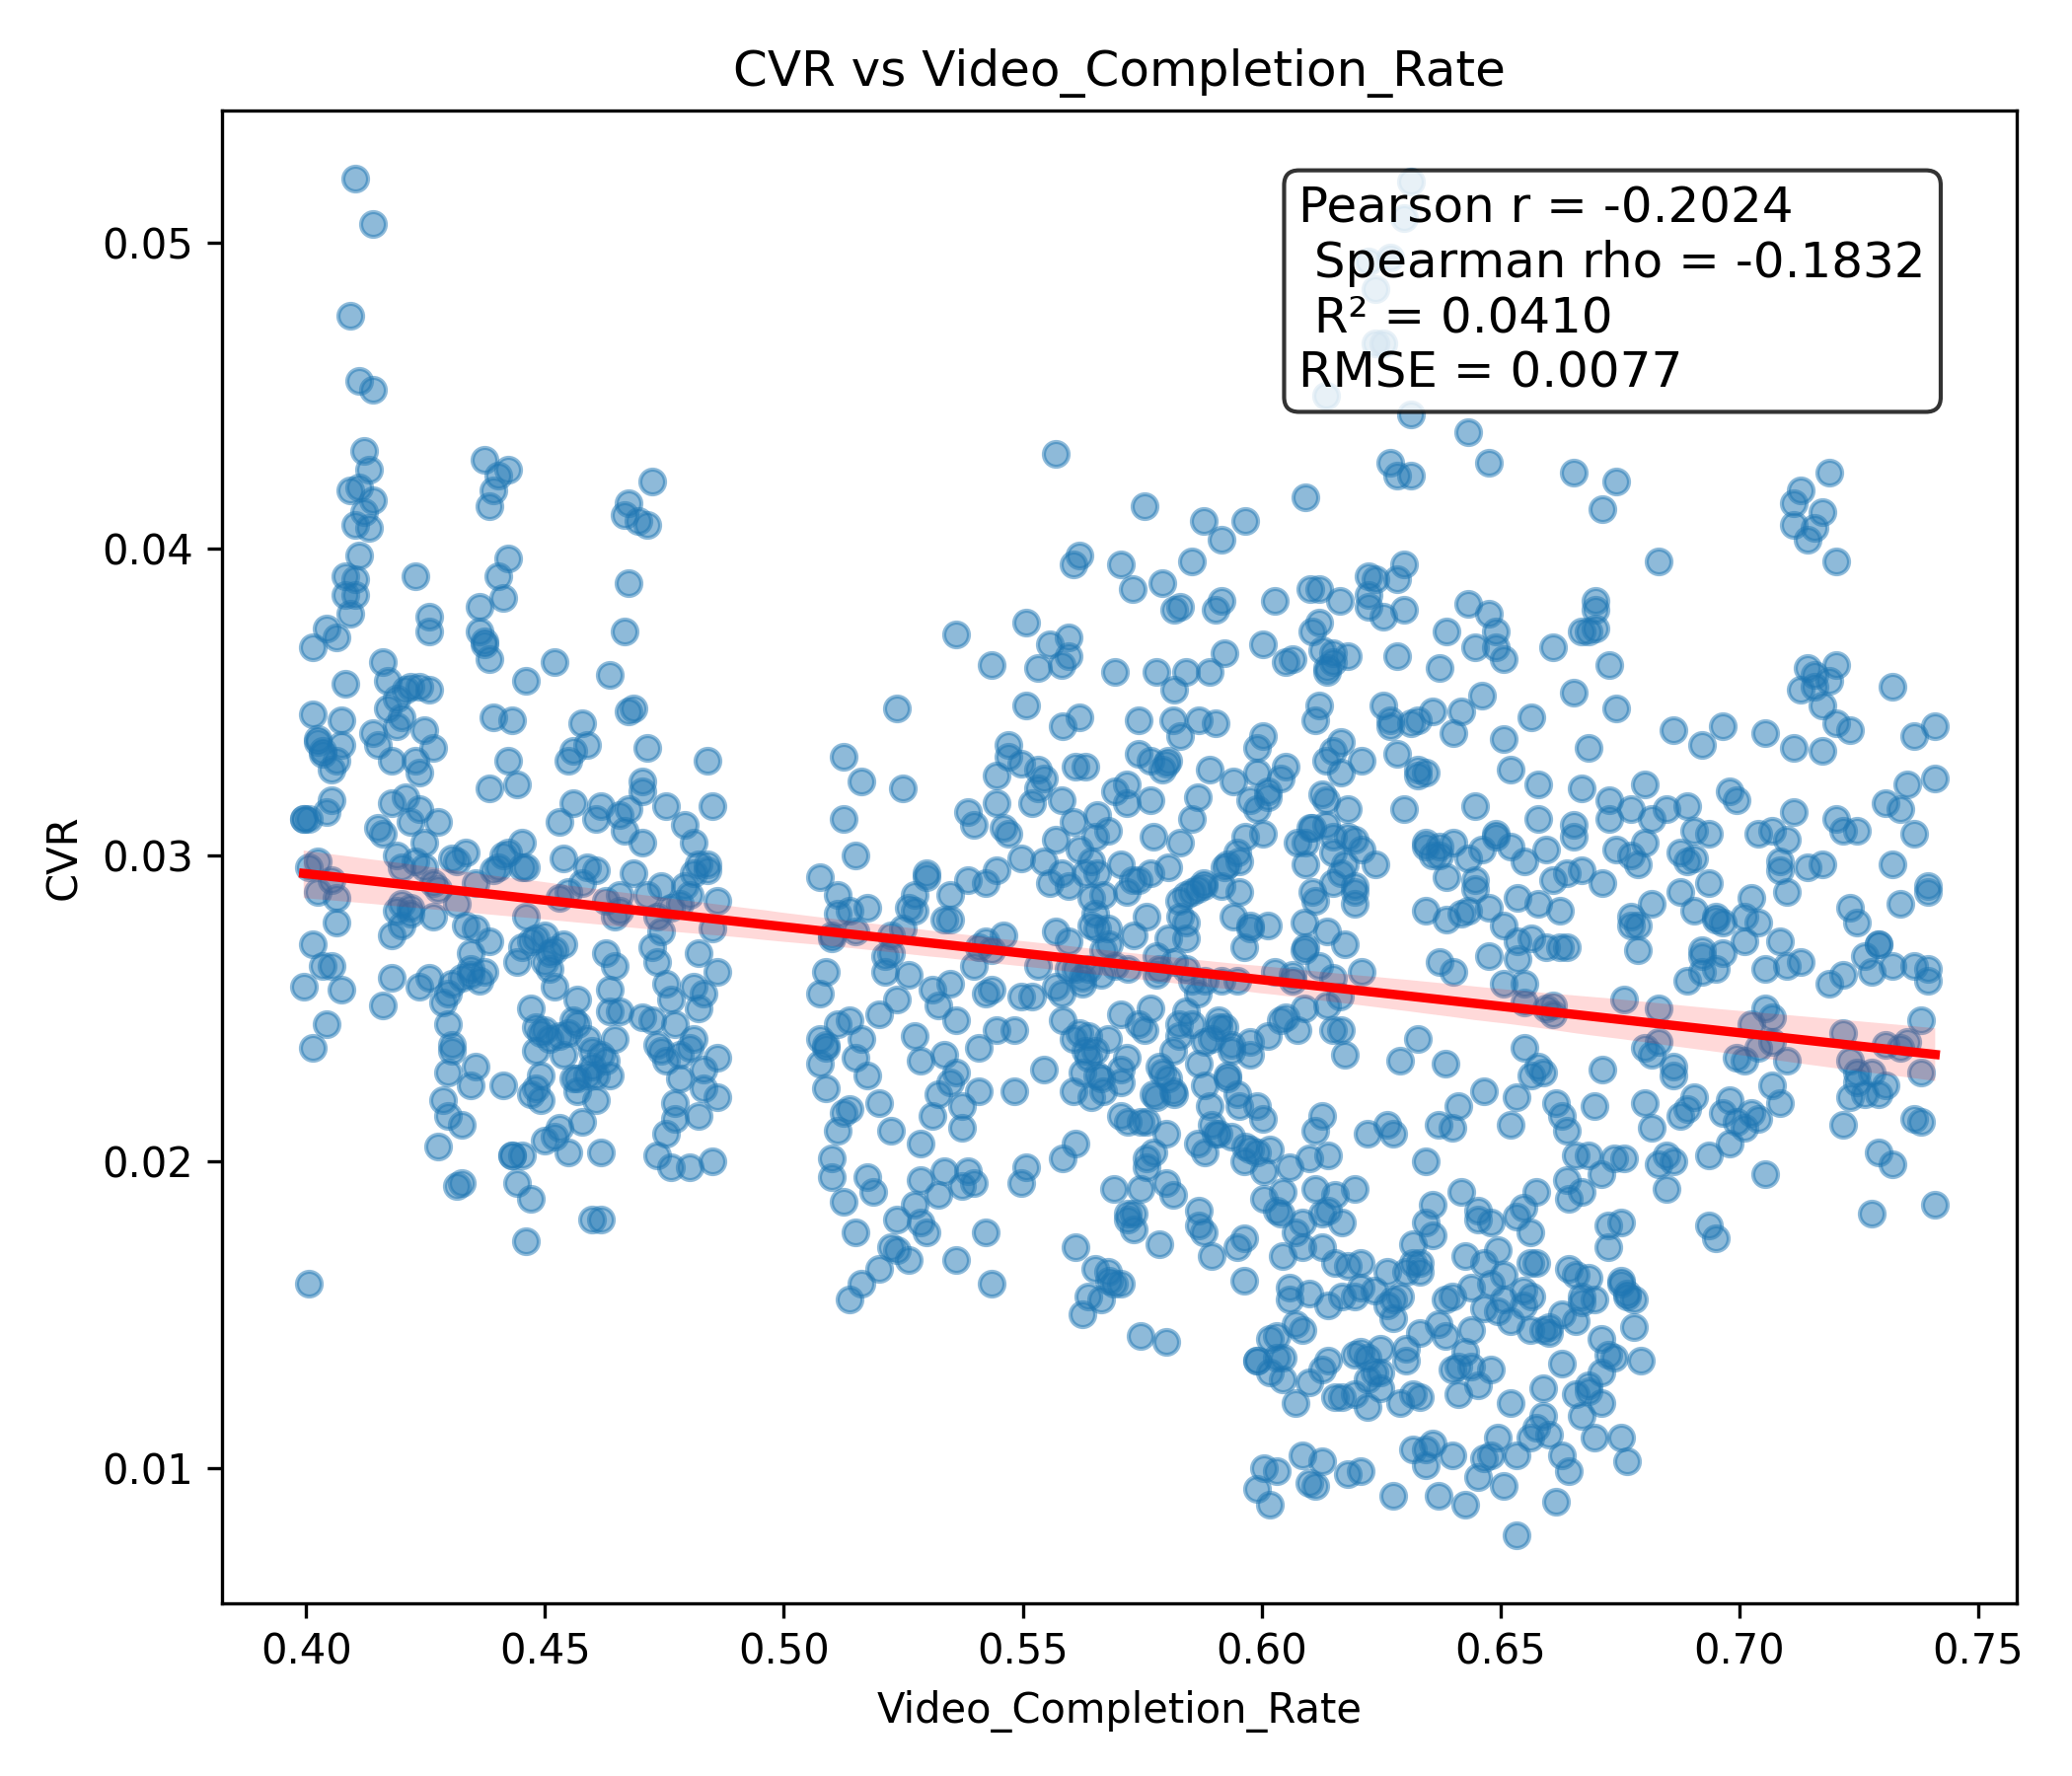
\includegraphics[width=0.7\textwidth]{images/CVR_vs_Video_Completion_Rate.png}
	\caption{CVR vs Video Completion Rate}
	\label{appendix:video_completion_rate}
\end{figure}

These results suggests that campaigns with higher video completion rates tend to exhibit slightly lower conversion rates. However, the magnitude of the relationship is weak, indicating that Video Completion Rate alone is not a strong predictor of Conversion rate.

\section{Relationship Between Video Completion Rate and Platform}
\label{appendix:video_completion_rate_platform_analysis}

\subsection{Video Completion Rate by Platform}
\label{appendix:video_completion_rate_platform_analysis_VCR}

\subsubsection{Descriptive Statistics}

\begin{table}[H]
	\centering
	\caption{Descriptive statistics for Video Completion Rate by platform.}
	\begin{tabular}{lcccc}
		\toprule
		Platform & Mean & Median & Std. Dev. & Count \\
		\midrule
		FB & 0.4430 & 0.4442 & 0.0250 & 299 \\
		TT & 0.6195 & 0.6163 & 0.0581 & 908 \\
		\bottomrule
	\end{tabular}
\end{table}

\subsubsection{Assumption Tests}

\subsubsection{Shapiro--Wilk Test}

\begin{table}[H]
	\centering
	\begin{tabular}{lc}
		\toprule
		Platform & p-value \\
		\midrule
		FB & $<0.0001$ \\
		TT & $<0.0001$ \\
		\bottomrule
	\end{tabular}
\end{table}

Both platform distributions significantly deviated from normality ($p<0.05$).

\vspace{0.3cm}

\subsubsection{Levene's Test}

\begin{table}[H]
	\centering
	\begin{tabular}{lc}
		\toprule
		Statistic & Value \\
		\midrule
		p-value & $<0.0001$ \\
		\bottomrule
	\end{tabular}
\end{table}

The variability of \textbf{Video Completion Rate differed significantly} between platforms. However, it is important to note that TT has 3 product\_categories while FB has 1, so the difference in STD may be attributed to TT having more diverse product categories.

\vspace{0.3cm}

\subsubsection{Kruskal--Wallis Test}

\begin{table}[H]
	\centering
	\begin{tabular}{lc}
		\toprule
		Statistic & Value \\
		\midrule
		H-statistic & 674.2412 \\
		p-value & $<0.0001$ \\
		\bottomrule
	\end{tabular}
\end{table}

The Kruskal--Wallis test indicates a statistically significant difference in Video Completion Rate between advertising platforms.

\vspace{0.3cm}

\subsubsection{Dunn Post-hoc Test}

\begin{table}[H]
	\centering
	\caption{Pairwise Dunn test p-values (Bonferroni adjusted).}
	\begin{tabular}{lcc}
		\toprule
		& FB & TT \\
		\midrule
		FB & -- & $<0.0001$ \\
		TT & $<0.0001$ & -- \\
		\bottomrule
	\end{tabular}
\end{table}

Facebook and TikTok exhibited statistically significant differences in Video Completion Rate, with TikTok achieving significantly higher completion rates than Facebook.

\subsubsection{Summary}

\begin{itemize}
	\item The \textbf{highest average Video Completion Rate} was achieved by \textbf{TikTok} (0.6195).
	\item The \textbf{lowest average Video Completion Rate} was observed for \textbf{Facebook} (0.4430).
	\item \textbf{TikTok achieved significantly higher Video Completion Rates than Facebook} ($p<0.05$).
\end{itemize}

\subsection{Video Completion Rate by TT Platform by Product Category}
\label{appendix:video_completion_rate_TT_platform_by_product}

\subsubsection{Descriptive Statistics}

\begin{table}[H]
	\centering
	\caption{Descriptive statistics for Video Completion Rate by product category.}
	\begin{tabular}{lcccc}
		\toprule
		Product Category & Mean & Median & Std. Dev. & Count \\
		\midrule
		Diet & 0.5618 & 0.5619 & 0.0320 & 293 \\
		Preworkout & 0.6181 & 0.6181 & 0.0349 & 300 \\
		Protein & 0.6745 & 0.6758 & 0.0387 & 315 \\
		\bottomrule
	\end{tabular}
\end{table}

\subsubsection{Assumption Tests}

\subsubsection{Shapiro--Wilk Test}

\begin{table}[H]
	\centering
	\begin{tabular}{lc}
		\toprule
		Product Category & p-value \\
		\midrule
		Diet & $<0.0001$ \\
		Preworkout & $<0.0001$ \\
		Protein & $<0.0001$ \\
		\bottomrule
	\end{tabular}
\end{table}

All product category distributions significantly deviated from normality ($p<0.05$).

\vspace{0.3cm}

\subsubsection{Levene's Test}

\begin{table}[H]
	\centering
	\begin{tabular}{lc}
		\toprule
		Statistic & Value \\
		\midrule
		p-value & 0.0001 \\
		\bottomrule
	\end{tabular}
\end{table}

The variability of \textbf{Video Completion Rate differed significantly} across product categories.

\vspace{0.3cm}

\subsubsection{Kruskal--Wallis Test}

\begin{table}[H]
	\centering
	\begin{tabular}{lc}
		\toprule
		Statistic & Value \\
		\midrule
		H-statistic & 587.1425 \\
		p-value & $<0.0001$ \\
		\bottomrule
	\end{tabular}
\end{table}

The Kruskal--Wallis test indicates statistically significant differences in Video Completion Rate across product categories.

\vspace{0.3cm}

\subsubsection{Dunn Post-hoc Test}

\begin{table}[H]
	\centering
	\caption{Pairwise Dunn test p-values (Bonferroni adjusted).}
	\begin{tabular}{lccc}
		\toprule
		& Diet & Preworkout & Protein \\
		\midrule
		Diet & -- & $<0.0001$ & $<0.0001$ \\
		Preworkout & $<0.0001$ & -- & $<0.0001$ \\
		Protein & $<0.0001$ & $<0.0001$ & -- \\
		\bottomrule
	\end{tabular}
\end{table}

All pairwise comparisons between product categories were statistically significant, indicating that each product category achieved a distinct level of Video Completion Rate.

\subsubsection{Within the TT Platform we have the following summary:}

\begin{itemize}
	\item The \textbf{highest average Video Completion Rate} was achieved by \textbf{Protein} (0.6745).
	\item The \textbf{lowest average Video Completion Rate} was observed for \textbf{Diet} (0.5618).
	\item \textbf{All product categories differed significantly} in Video Completion Rate ($p<0.05$), with Protein achieving the highest completion rates, followed by Preworkout and Diet.
\end{itemize}

\subsection{Video Completion Rate by Region}
\label{appendix:video_completion_rate_region_analysis_VCR}

\subsubsection{Descriptive Statistics}

\begin{table}[H]
	\centering
	\caption{Descriptive statistics for Video Completion Rate by region.}
	\begin{tabular}{lcccc}
		\toprule
		Region & Mean & Median & Std. Dev. & Count \\
		\midrule
		Midwest & 0.6206 & 0.6188 & 0.0584 & 220 \\
		Northeast & 0.6191 & 0.6165 & 0.0578 & 229 \\
		South & 0.6199 & 0.6160 & 0.0587 & 228 \\
		West & 0.6184 & 0.6140 & 0.0580 & 231 \\
		\bottomrule
	\end{tabular}
\end{table}

\subsubsection{Assumption Tests}

\subsubsection{Shapiro--Wilk Test}

\begin{table}[H]
	\centering
	\begin{tabular}{lc}
		\toprule
		Region & p-value \\
		\midrule
		Midwest & 0.0096 \\
		Northeast & 0.0090 \\
		South & 0.0028 \\
		West & 0.0065 \\
		\bottomrule
	\end{tabular}
\end{table}

All regional distributions significantly deviated from normality ($p<0.05$).

\vspace{0.3cm}

\subsubsection{Levene's Test}

\begin{table}[H]
	\centering
	\begin{tabular}{lc}
		\toprule
		Statistic & Value \\
		\midrule
		p-value & 0.9766 \\
		\bottomrule
	\end{tabular}
\end{table}

No statistically significant difference in the variability of \textbf{Video Completion Rate} was observed across regions.

\vspace{0.3cm}

\subsubsection{Kruskal--Wallis Test}

\begin{table}[H]
	\centering
	\begin{tabular}{lc}
		\toprule
		Statistic & Value \\
		\midrule
		H-statistic & 0.1893 \\
		p-value & 0.9793 \\
		\bottomrule
	\end{tabular}
\end{table}

The Kruskal--Wallis test indicates that there are no statistically significant differences in Video Completion Rate across regions.

\subsubsection{Summary}

\begin{itemize}
	\item The \textbf{highest average Video Completion Rate} was achieved by the \textbf{Midwest} (0.6206).
	\item The \textbf{lowest average Video Completion Rate} was observed for the \textbf{West} (0.6184).
	\item \textbf{No statistically significant differences} in Video Completion Rate were observed across regions ($p \geq 0.05$).
\end{itemize}

\subsection{Video Completion Rate by Competitive Event}
\label{appendix:video_completion_rate_competitive_event_analysis_VCR}

\subsubsection{Descriptive Statistics}

\begin{table}[H]
	\centering
	\caption{Descriptive statistics for Video Completion Rate by competitive event status.}
	\begin{tabular}{lcccc}
		\toprule
		Competitive Event & Mean & Median & Std. Dev. & Count \\
		\midrule
		False & 0.6189 & 0.6152 & 0.0580 & 872 \\
		True & 0.6335 & 0.6195 & 0.0610 & 36 \\
		\bottomrule
	\end{tabular}
\end{table}

\subsubsection{Assumption Tests}

\subsubsection{Shapiro--Wilk Test}

\begin{table}[H]
	\centering
	\begin{tabular}{lc}
		\toprule
		Competitive Event & p-value \\
		\midrule
		False & $<0.0001$ \\
		True & 0.0273 \\
		\bottomrule
	\end{tabular}
\end{table}

Both distributions significantly deviated from normality ($p<0.05$).

\vspace{0.3cm}

\subsubsection{Levene's Test}

\begin{table}[H]
	\centering
	\begin{tabular}{lc}
		\toprule
		Statistic & Value \\
		\midrule
		p-value & 0.9008 \\
		\bottomrule
	\end{tabular}
\end{table}

No statistically significant difference in the variability of \textbf{Video Completion Rate} was observed between competitive and non-competitive event periods.

\vspace{0.3cm}

\subsubsection{Kruskal--Wallis Test}

\begin{table}[H]
	\centering
	\begin{tabular}{lc}
		\toprule
		Statistic & Value \\
		\midrule
		H-statistic & 1.5983 \\
		p-value & 0.2061 \\
		\bottomrule
	\end{tabular}
\end{table}

The Kruskal--Wallis test indicates that there are no statistically significant differences in Video Completion Rate between competitive and non-competitive event periods.

\subsubsection{Summary}

\begin{itemize}
	\item The \textbf{highest average Video Completion Rate} was observed during \textbf{competitive events} (0.6335).
	\item The \textbf{lowest average Video Completion Rate} was observed during \textbf{non-competitive event periods} (0.6189).
	\item \textbf{No statistically significant difference} in Video Completion Rate was observed between competitive and non-competitive event periods ($p \geq 0.05$).
\end{itemize}

\begin{figure}[H]
	\centering
	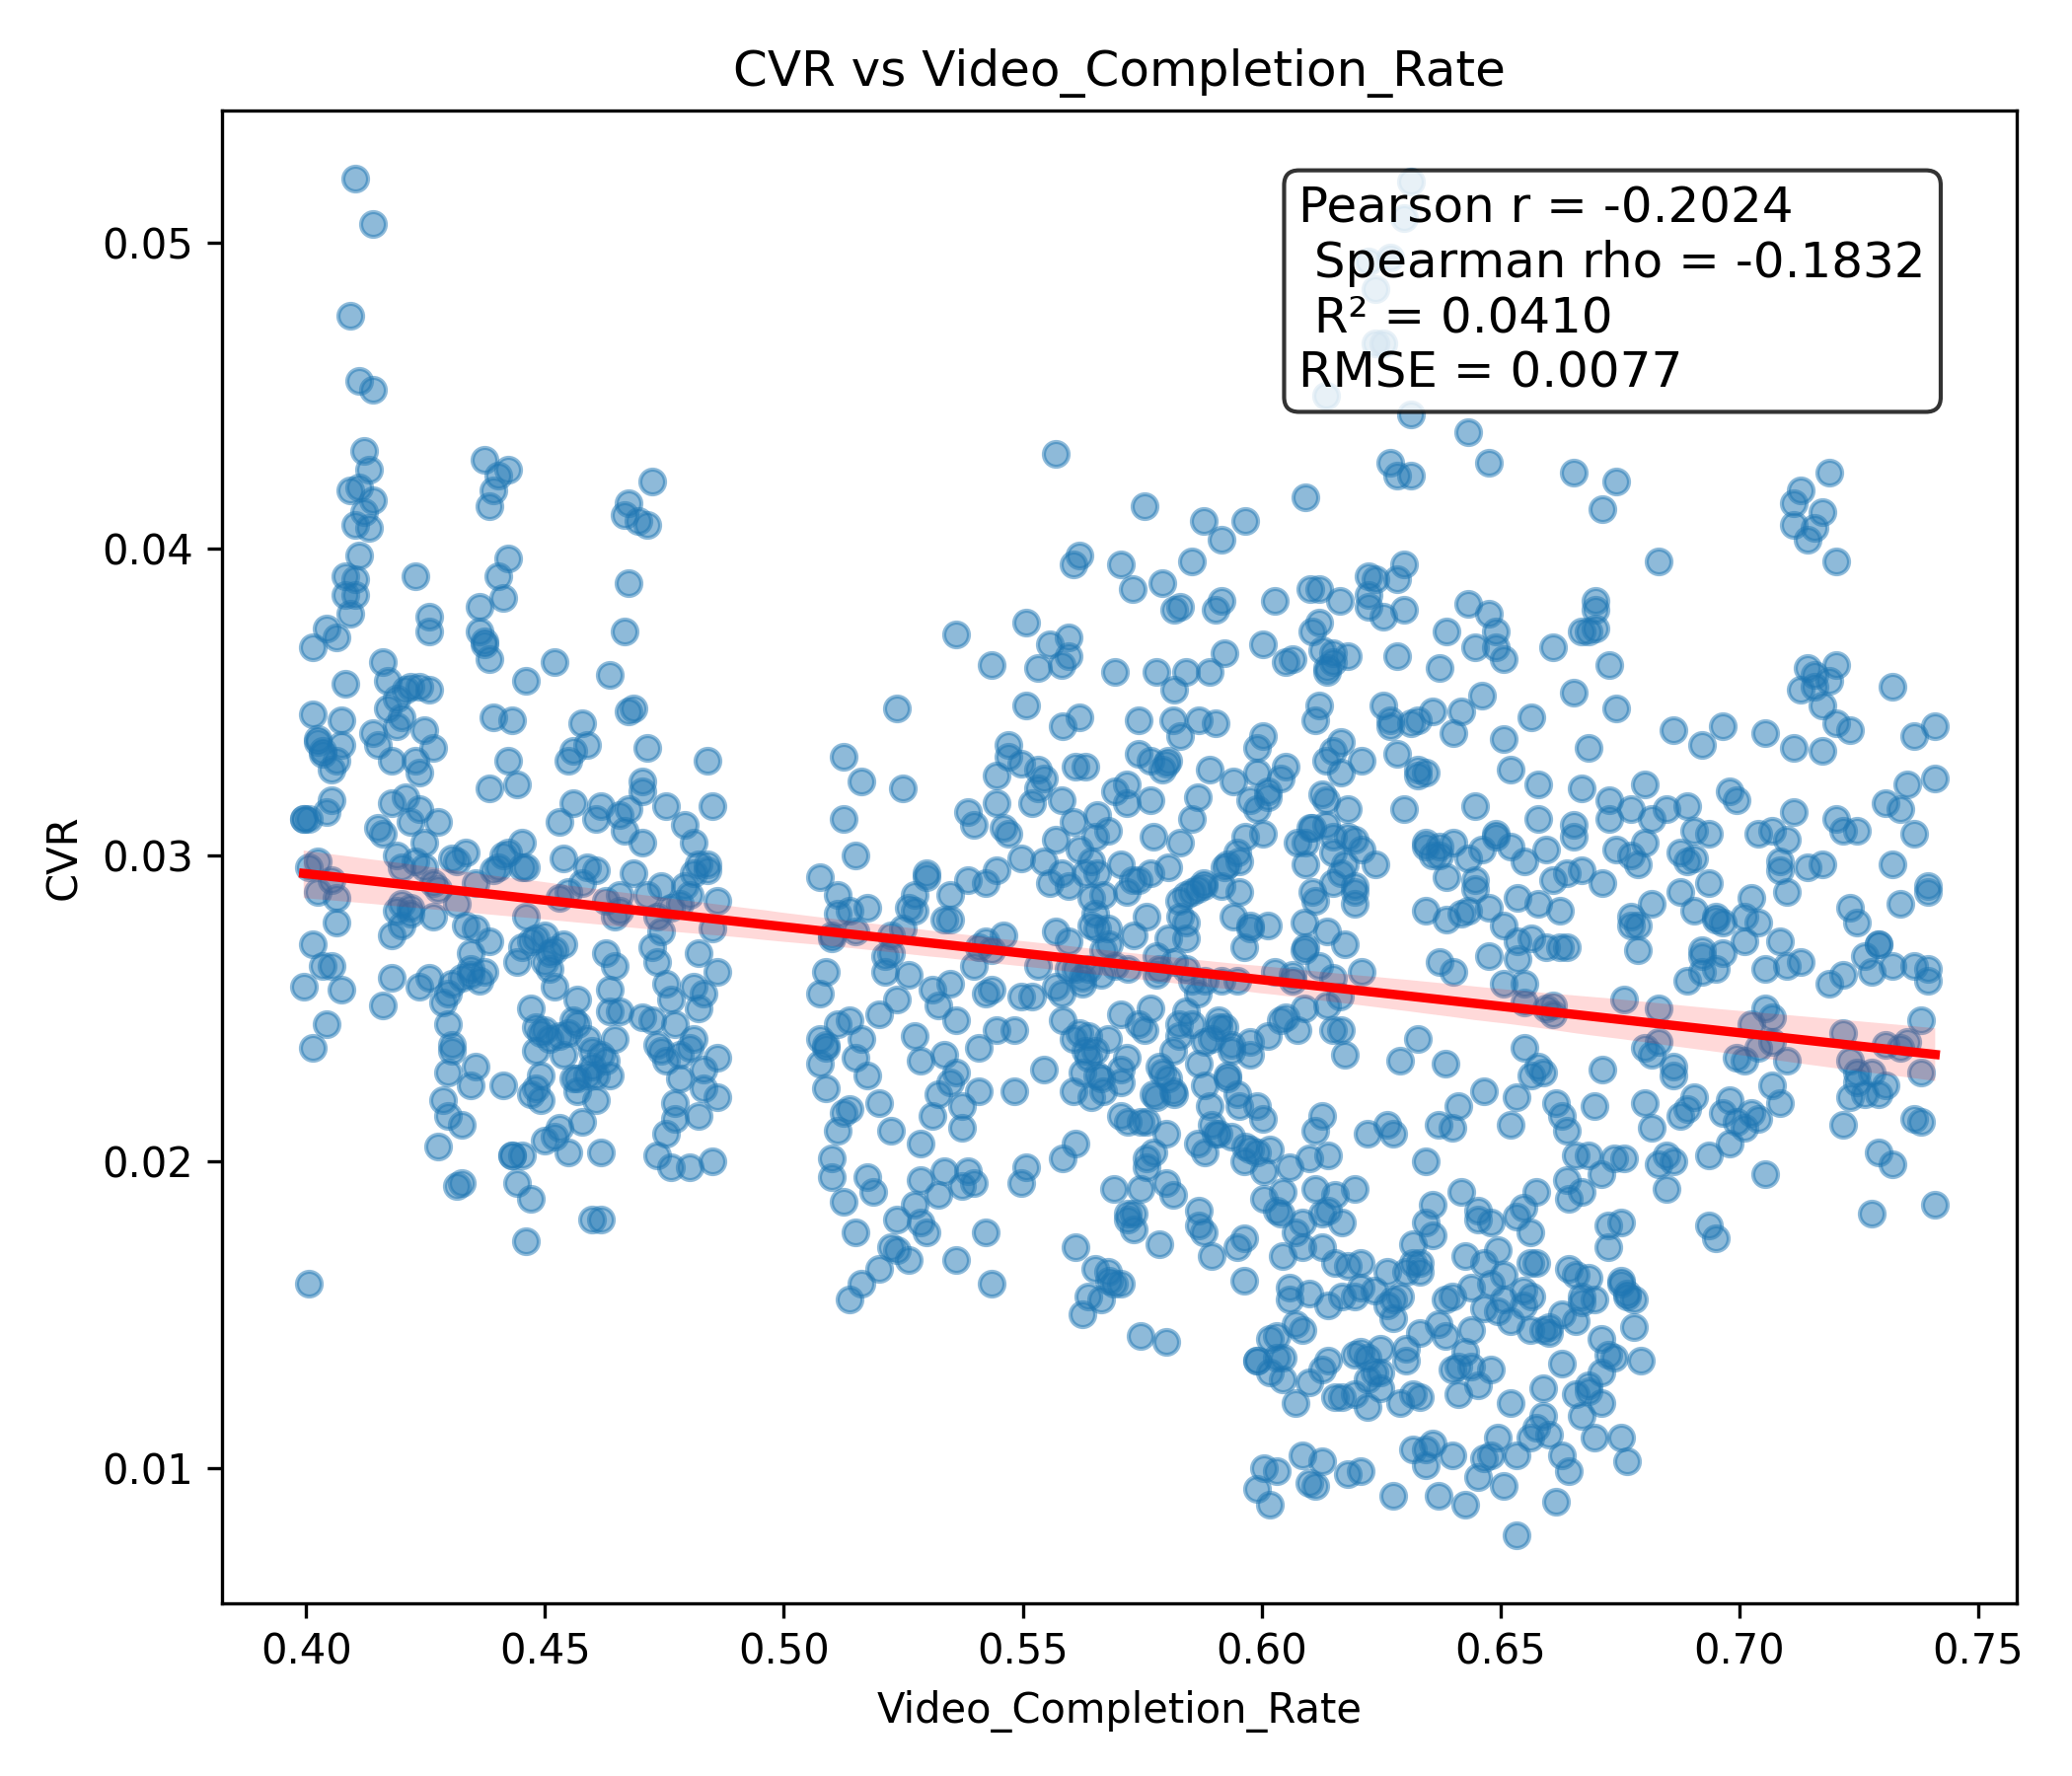
\includegraphics[width=0.7\textwidth]{images/CVR_vs_Video_Completion_Rate.png}
	\caption{CVR vs Video Completion Rate}
	\label{appendix:video_completion_rate_by_platfor}
\end{figure}



%\subsection{Video Com}
\subsection{Summary for Video Completion Rate by Platform}
\begin{figure}[H]
	\centering
	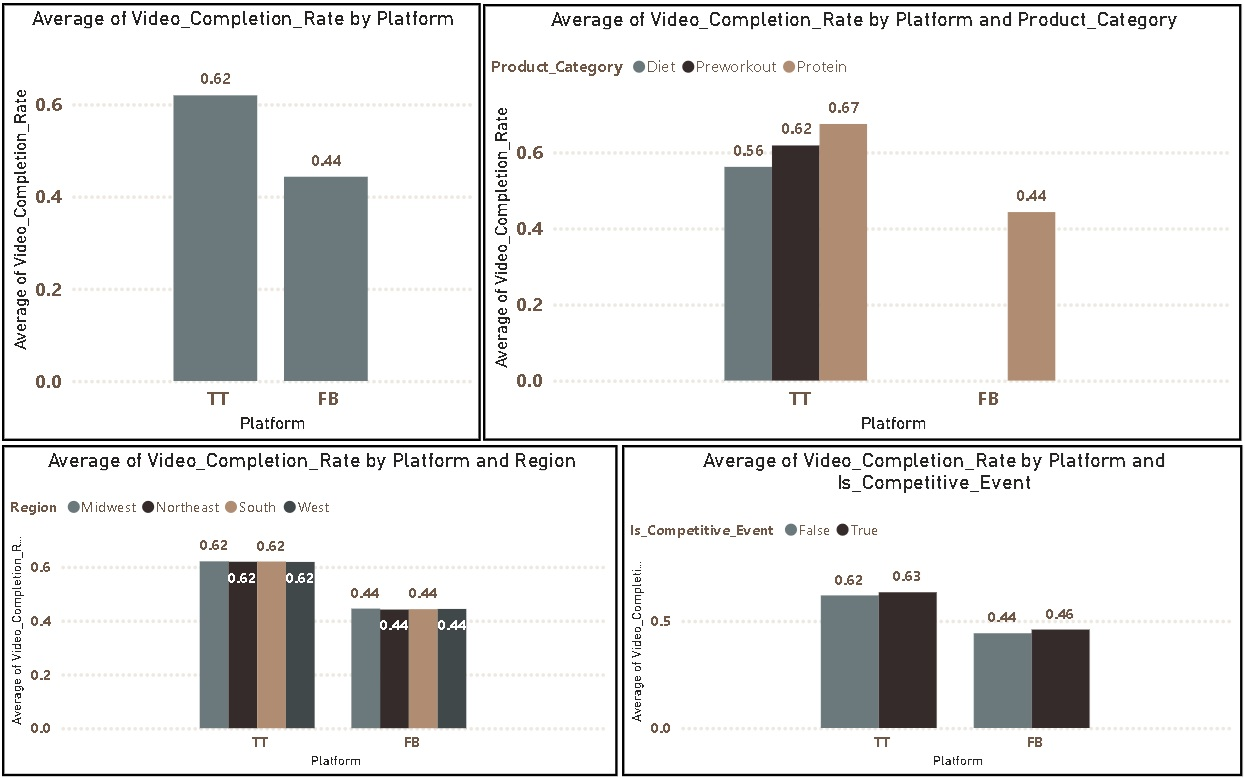
\includegraphics[width=1\textwidth]{images/video_completion_by_platform_by.jpg}
	\caption{Scatter plots of CVR versus Video Completion Rate grouped by platform, product category, competitive event status, and region}
	\label{fig:video_completion_rate_categorized}
\end{figure}

\begin{itemize}
	
	\item Video ads from TT platform exhibited higher video completion rate for Protein product category [Appendix \ref{appendix:video_completion_rate_platform_analysis_VCR}].
	
	\item Within the TT platform, product category seem to significantly affect video completion rate where Protein product exhibits the highest video completion rate [Appendix \ref{appendix:video_completion_rate_TT_platform_by_product}].
	
	\item Further tests, like FB video ads with Preworkout and Diet product categories are needed for evidence of Platform effects to video completion rate.
	
	\item Competitive events and Region seem to not affect the video completion rate across TT and FB Platforms.
\end{itemize}

Overall, product categories and platform(potentially) significantly affect video completion rate. These insights will be helpful for campaigns with a goal of maximizing video completion rate.





\end{document}